\documentclass[11pt, a4paper]{article}
\usepackage[utf8]{inputenc}
\usepackage{graphicx}
\usepackage{amsmath}
\usepackage{geometry}
\geometry{margin=1in}
\usepackage{float}
\usepackage{caption}
\usepackage{booktabs}
\usepackage{hyperref}

\title{\textbf{Electronic Devices \& Circuits Laboratory (EE2301)} \\
\Large Experiment 6: NMOS Source Follower with Current-Mirror Load}
\author{Bhargav K (EE25BTECH11013) \\ Aditya Appana (EE25BTECH11004)}
\date{\today}

\begin{document}
\maketitle

\section{Objective}
To assemble and experimentally characterize an NMOS source follower (common-drain amplifier) biased by an active current-source load constructed from an NMOS current mirror using a $V_{DD} = 10\text{ V}$ laboratory DC source. The specific objectives are:
\begin{enumerate}
    \item Verify the current mirror reference branch and establish a stable $\approx 33\text{--}34\text{ mA}$ tail current under the $10\text{ V}$ power supply.
    \item Measure the large-signal DC transfer characteristic ($V_{out}$ vs.\ $V_{in}$), determine the linear voltage tracking range, and extract the gate-to-source DC level shift ($V_{GS}$).
    \item Investigate operating limits, specifically the triode boundary at low $V_{in}$ and thermal runaway effects observed in the active current-mirror transistor at higher input voltages.
    \item Characterize the small-signal AC voltage gain ($A_v$) across a frequency range from 6~Hz to 100~kHz.
    \item Measure the small-signal output resistance ($R_{out}$) using capacitively coupled discrete resistive loads and compare the extracted value with weak-inversion theoretical predictions adjusted for the 10~V operating rail.
\end{enumerate}

\section{Components and Equipment Required}
The hardware components and laboratory test instruments specified in Section~2 of the lab manual and utilized during the experiment are listed in Table~\ref{tab:components}.

\begin{table}[H]
    \centering
    \small
    \begin{tabular}{lp{8.5cm}c}
        \toprule
        \textbf{Item} & \textbf{Specification / Description} & \textbf{Qty} \\
        \midrule
        MOSFET & Vishay SI9926BDY, dual N-channel, SO-8 on DIP breakout & 2 \\
               & (3 channels used: $M_{ref}$, $M_{cs}$, $M_{sf}$; 1 spare channel) & \\
        Reference Resistor $R_{ref}$ & $270\ \Omega$, $\pm 5\%$, $0.5\text{ W}$ metal film & 1 \\
        DC Bias Potentiometer & $10\text{ k}\Omega$, multi-turn cermet trimmer (for $V_{in}$ DC bias) & 1 \\
        Decoupling Resistor $R_{bias}$ & $1\text{ M}\Omega$, isolates AC signal path from bias potentiometer & 1 \\
        Coupling Capacitor $C_{in}$ & $1\ \mu\text{F}$ electrolytic, AC-couples function generator & 1 \\
        Load Resistors & Nominal 10~$\Omega$, 47~$\Omega$, 100~$\Omega$ (measured 10.2~$\Omega$, 47.0~$\Omega$, 112.0~$\Omega$) & 1 each \\
        DC Power Supply & Regulated $0\text{--}30\text{ V}$, set to $10.0\text{ V}$, current-limited to $150\text{ mA}$ & 1 \\
        Function Generator & Sine wave output, small amplitude, $10\text{ Hz}\text{--}100\text{ kHz}$ sweep & 1 \\
        Digital Oscilloscope & Tektronix 2-channel DSO, to view $V_{in}$ and $V_{out}$ simultaneously & 1 \\
        Digital Multimeter (DMM) & 4.5-digit bench DMM for DC transfer measurements & 2 \\
        Breadboard \& Jumpers & Standard solderless breadboard and connection wires & as req. \\
        Datasheet & Vishay SI9926BDY datasheet (provided laboratory reference copy) & 1 \\
        \bottomrule
    \end{tabular}
    \caption{Components and Laboratory Equipment Required (Lab Manual Section 2).}
    \label{tab:components}
\end{table}

\section{Circuit Diagram and Simulation Setup}
The circuit consists of two main stages: a current mirror providing active current-source biasing, and the common-drain follower transistor $M_{sf}$ ($M_1$). Across the two SI9926BDY dual-MOSFET packages, three identical NMOS channels were assigned:
\begin{itemize}
    \item \textbf{Channel 1 ($M_{ref}$ / $M_3$):} Diode-connected reference transistor tied to $V_{DD} = 10\text{ V}$ through $R_{ref} = 270\ \Omega$.
    \item \textbf{Channel 2 ($M_{cs}$ / $M_2$):} Current-mirror transistor acting as the active tail load for the source follower.
    \item \textbf{Channel 3 ($M_{sf}$ / $M_1$):} Source follower whose drain connects directly to $V_{DD} = 10\text{ V}$, gate to $V_{in}$, and source to the output node $V_{out}$.
\end{itemize}

The breadboard hardware assembly and the corresponding LTspice simulation schematic are shown in Figure~\ref{fig:breadboard} and Figure~\ref{fig:ltspice_schematic}.

\begin{figure}[H]
    \centering
    \begin{minipage}{0.48\textwidth}
        \centering
        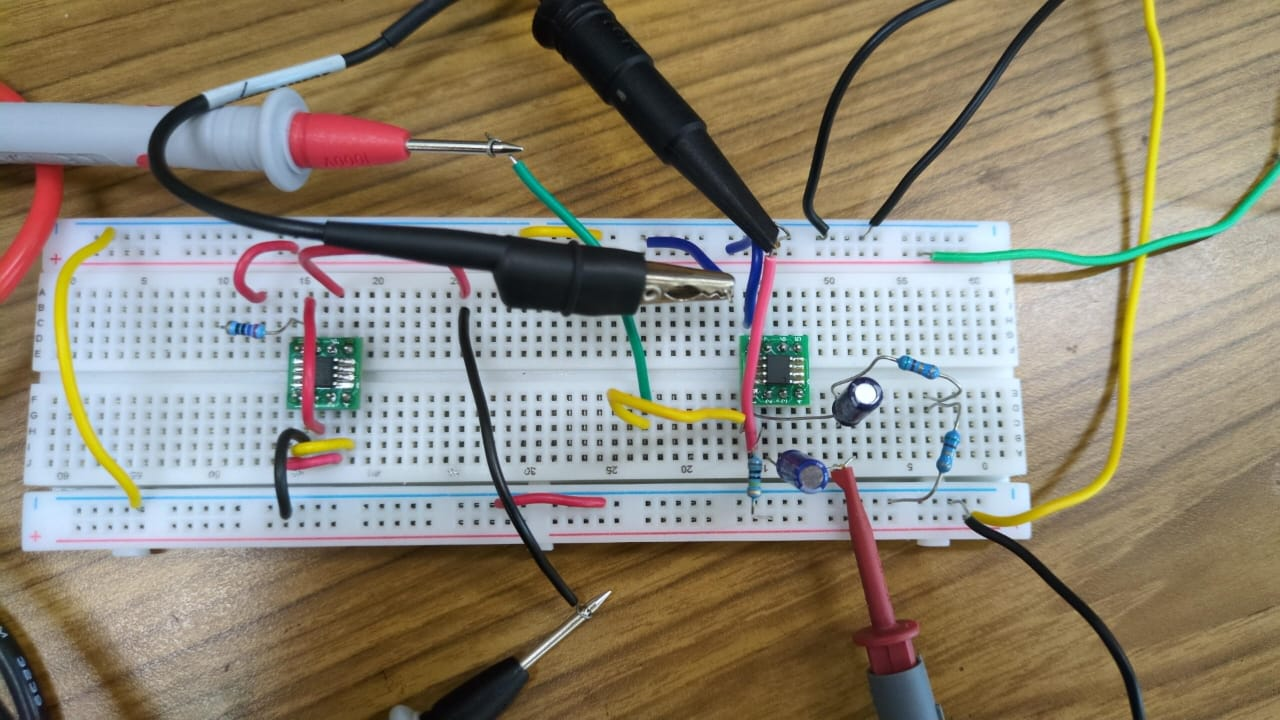
\includegraphics[width=\linewidth]{originalcircuit.jpeg}
        \caption{Breadboard Experimental Setup.}
        \label{fig:breadboard}
    \end{minipage}\hfill
    \begin{minipage}{0.48\textwidth}
        \centering
        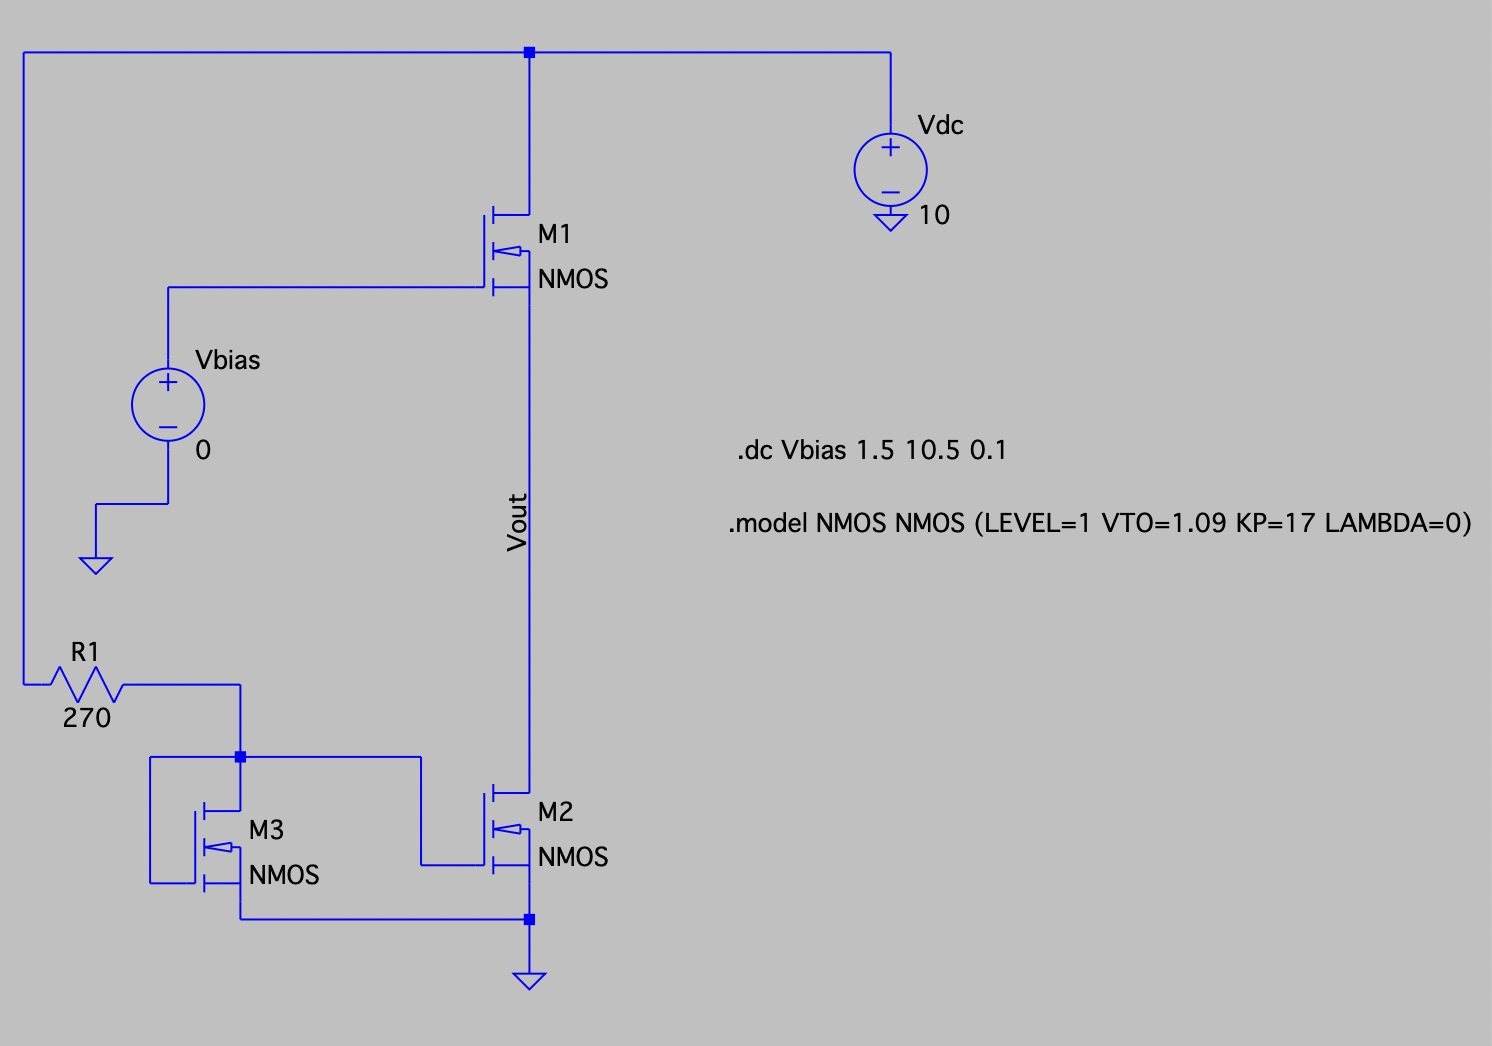
\includegraphics[width=\linewidth]{ckt_dc.png}
        \caption{LTspice Simulation Schematic ($V_{DD} = 10\text{ V}$).}
        \label{fig:ltspice_schematic}
    \end{minipage}
\end{figure}

The DC simulation schematic (Figure~\ref{fig:ltspice_schematic}) incorporates a Level-1 NMOS model calibrated to the SI9926BDY bench measurements ($V_{TO} = 1.09\text{ V}$, $K_P = 17\text{ A/V}^2$, $V_{DD} = 10\text{ V}$) and executes a DC sweep of $V_{in}$ from 1.5~V to 10.5~V in 0.1~V increments. The corresponding AC simulation schematic with input coupling network is presented in Figure~\ref{fig:sim_ac}(a).

\section{Theoretical Background and Analysis}

\subsection{Current Mirror Reference Current}
With the laboratory power supply set to $V_{DD} = 10\text{ V}$ and reference resistor $R_{ref} = 270\ \Omega$, the diode-connected transistor $M_{ref}$ establishes the reference current:
\begin{equation}
I_{ref} = \frac{V_{DD} - V_{GS(M_{ref})}}{R_{ref}} \approx \frac{10\text{ V} - 1.09\text{ V}}{270\ \Omega} \approx 33.0\text{ mA}
\end{equation}
(or $I_{ref} \approx \frac{10\text{ V} - 0.85\text{ V}}{270\ \Omega} \approx 33.9\text{ mA}$ using the experimentally observed level shift $V_{GS} \approx 0.85\text{ V}$). Note that while Section~9 of the laboratory manual assumes a nominal $12\text{ V}$ rail ($I_{ref} \approx 40.4\text{ mA}$), our bench setup employed $V_{DD} = 10\text{ V}$, scaling the reference current down to $\approx 33\text{--}34\text{ mA}$. This closely matches the initial mirror current measured on the bench ($34.30\text{ mA}$ at $V_{in} = 2.0\text{ V}$). Since $M_{cs}$ mirrors the gate voltage of $M_{ref}$ 1:1, it forces this tail current $I_{cs}$ through the follower stage.

\subsection{Large-Signal DC Transfer Function and Dynamic Range}
The follower transistor $M_{sf}$ carries the tail current set by $M_{cs}$: $I_{D1} = I_{cs} \approx I_{ref}$. Because this current is constant, the gate-to-source voltage $V_{GS1}$ remains locked to a single operating value. Applying KVL around the gate-source loop:
\begin{equation}
V_{out} = V_{in} - V_{GS1}(I_{ref})
\end{equation}
Differentiating with respect to $V_{in}$ yields an ideal transfer slope:
\begin{equation}
\frac{dV_{out}}{dV_{in}} = 1.00\text{ V/V}
\end{equation}
The output directly tracks the input with a fixed downward level shift equal to $V_{GS1} \approx 1.09\text{ V}$ (or $0.85\text{ V}$ measured). In Section~9 of the manual, theoretical $V_{out}$ values are tabulated assuming $V_{out,pred} = V_{in} - 1.09\text{ V}$ (spanning from $0.41\text{ V}$ at $1.5\text{ V}$ up to $9.41\text{ V}$ at $10.5\text{ V}$).

\noindent\textbf{Comparison with Differential Pair:} Unlike the differential amplifier characterized in Experiment 4 (which was strictly constrained to a narrow linear differential input window of roughly $\pm 150\text{ mV}$), the source follower provides an exceptionally wide linear range spanning from approximately $V_{in} \approx 1.5\text{ V}$ up toward the positive supply rail ($10\text{ V}$).

\subsection{Small-Signal Voltage Gain}
From the small-signal equivalent model:
\begin{equation}
A_v = \frac{v_{out}}{v_{in}} = \frac{g_{m1}}{g_{m1} + g_{mb1} + \frac{1}{r_{o1}} + \frac{1}{r_{o2}}} = \frac{g_{m1}}{g_{m1} + g_{mb1} + g_{o,total}}
\end{equation}
Because the source and body are internally bonded together in each channel of the SI9926BDY breakout adapter, the source-to-body voltage is zero ($V_{SB} = 0$), eliminating the body effect ($g_{mb1} = 0$). Furthermore, since the transconductance $g_{m1} \approx 0.85\text{ A/V}$ far exceeds the output conductances $g_{o,total} \approx 1/r_{o1} + 1/r_{o2}$, the voltage gain evaluates to near-unity:
\begin{equation}
A_v \approx 1.00\text{ V/V} \quad (0\text{ dB})
\end{equation}

\subsection{Small-Signal Output Resistance}
Looking back into the source terminal of $M_1$, the small-signal output resistance is:
\begin{equation}
R_{out} = \frac{1}{g_{m1}} \parallel r_{o1} \parallel r_{o2} \approx \frac{1}{g_{m1}}
\end{equation}
Operating in weak inversion at $I_{ref} \approx 33.0\text{ mA}$ (under $V_{DD} = 10\text{ V}$), the transconductance is governed by exponential subthreshold physics:
\begin{equation}
g_{m1} = \frac{I_{ref}}{n V_T} \approx \frac{33.0\text{ mA}}{1.5 \times 26\text{ mV}} \approx 0.846\text{ A/V}
\end{equation}
(or $g_{m1} \approx 0.869\text{ A/V}$ with $I_{ref} \approx 33.9\text{ mA}$). This yields the 10~V adjusted theoretical output resistance:
\begin{equation}
R_{out, theoretical} \approx \frac{1}{0.846\text{ A/V}} \approx 1.18\ \Omega
\end{equation}
(compared to the manual's nominal $0.96\ \Omega$ which assumed $V_{DD} = 12\text{ V}$, $I_{ref} \approx 40.4\text{ mA}$).

\subsection{Frequency Response and Bandwidth Mechanics}
The lab manual emphasizes distinguishing input-coupling roll-off from output-side bandwidth limits:
\begin{itemize}
    \item \textbf{Output Pole:} Because $R_{out} \approx 1.87\ \Omega$ is exceptionally small, the pole formed by the output node and any load capacitance $C_L$, $f_{p,out} = \frac{1}{2\pi R_{out} C_L}$, is pushed well beyond several tens of megahertz. Hence, no high-frequency roll-off can occur in the audio or ultrasonic sweep range (up to 100~kHz).
    \item \textbf{Input Pole:} The AC input path contains a high-pass coupling network ($C_{in} = 1\ \mu\text{F}$ and $R_{bias} = 1\text{ M}\Omega$). Any minor attenuation observed at single-digit frequencies (6--10~Hz) originates strictly from this input coupling filter ($f_L \approx \frac{1}{2\pi R_{bias} C_{in}}$), rather than any intrinsic limitation of the source follower itself.
\end{itemize}

\section{Experimental Procedure}
\begin{enumerate}
    \item \textbf{Mirror Verification (Section 6.1):} Assembled the reference branch ($R_{ref} = 270\ \Omega$, $M_{ref}$) and the mirror device $M_{cs}$ with $M_{sf}$ gate left disconnected. Set the DC bench power supply to $V_{DD} = 10\text{ V}$ with a $150\text{ mA}$ current limit. Measured the voltage drop across $R_{ref}$ and confirmed $I_{ref} = V_{Rref}/R_{ref} \approx 33\text{--}34\text{ mA}$.
    \item \textbf{DC Transfer Characteristic (Section 6.2):} Connected $M_{sf}$ drain to $V_{DD} = 10\text{ V}$ and source to the $M_{cs}$ drain node ($V_{out}$). Swept the DC input voltage $V_{in}$ from 1.0~V to 8.5~V using the 10~k$\Omega$ potentiometer, simultaneously recording $V_{out}$ and the tail current $I_{cs}$.
    \item \textbf{Small-Signal Gain Setup (Section 6.3):} While the lab manual suggests setting $V_{in}$ DC bias to $\approx 7\text{ V}$ (mid-range of a 12~V rail), in our 10~V configuration $7\text{ V}$ sits near the positive rail where transistor dissipation is high ($I_{cs} \approx 77\text{ mA}$). Hence, a thermally safe bias of $V_{in,DC} = 3.0\text{ V}$ ($I_{cs} = 41.9\text{ mA}$) was selected. Added the $1\ \mu\text{F}$ coupling capacitor and $1\text{ M}\Omega$ isolation resistor. Applied a $200\text{ mV}_{p-p}$ sinusoidal input at 1~kHz from the function generator and measured $V_{in}$ and $V_{out}$ on the oscilloscope.
    \item \textbf{Frequency Response Sweep (Section 6.4):} Kept the input amplitude constant at $200\text{ mV}_{p-p}$ and swept test frequencies from 6~Hz to 100~kHz, measuring the output peak-to-peak amplitude at each frequency step.
    \item \textbf{Output Resistance via Loading (Section 6.5):} Connected load resistors ($10.2\ \Omega$, $47.0\ \Omega$, $112.0\ \Omega$) in turn from $V_{out}$ to ground through an AC-coupling blocking capacitor to isolate DC bias. Recorded loaded amplitudes and extracted $R_{out}$.
\end{enumerate}

\section{Experimental Observations and Results}

\subsection{DC Transfer Characteristic and Thermal Analysis (Table 1)}
The complete DC transfer dataset recorded in the laboratory notebook (from \texttt{EDC 7.xlsx}) is presented in Table~\ref{tab:dc_data}.

\begin{table}[H]
    \centering
    \small
    \setlength{\tabcolsep}{4.2pt}
    \begin{tabular}{cccc|cccc}
        \toprule
        \textbf{$V_{in}$ (V)} & \textbf{$V_{out}$ (V)} & \textbf{$V_{in} - V_{out}$ (V)} & \textbf{$I_{cs}$ (mA)} &
        \textbf{$V_{in}$ (V)} & \textbf{$V_{out}$ (V)} & \textbf{$V_{in} - V_{out}$ (V)} & \textbf{$I_{cs}$ (mA)} \\
        \midrule
        1.0 & 0.184 & 0.816 & 18.45 & 5.0 & 4.126 & 0.874 & 57.06 \\
        1.5 & 0.660 & 0.840 & 29.47 & 5.5 & 4.622 & 0.878 & 61.45 \\
        2.0 & 1.158 & 0.842 & 34.30 & 6.0 & 5.115 & 0.885 & 66.19 \\
        2.5 & 1.653 & 0.847 & 38.24 & 6.5 & 5.607 & 0.893 & 71.31 \\
        3.0 & 2.150 & 0.850 & 41.90 & 7.0 & 6.090 & 0.910 & 77.10 \\
        3.5 & 2.645 & 0.855 & 45.48 & 7.5 & 6.580 & 0.920 & 83.80 \\
        4.0 & 3.139 & 0.861 & 49.15 & 8.0 & 7.060 & 0.940 & 91.48 \\
        4.5 & 3.633 & 0.867 & 52.99 & 8.5 & 7.550 & 0.950 & 101.45 \\
        \bottomrule
    \end{tabular}
    \caption{Measured DC Transfer Characteristic and Tail Current (from EDC 7.xlsx)}
    \label{tab:dc_data}
\end{table}

\begin{figure}[H]
    \centering
    \begin{minipage}{0.48\textwidth}
        \centering
        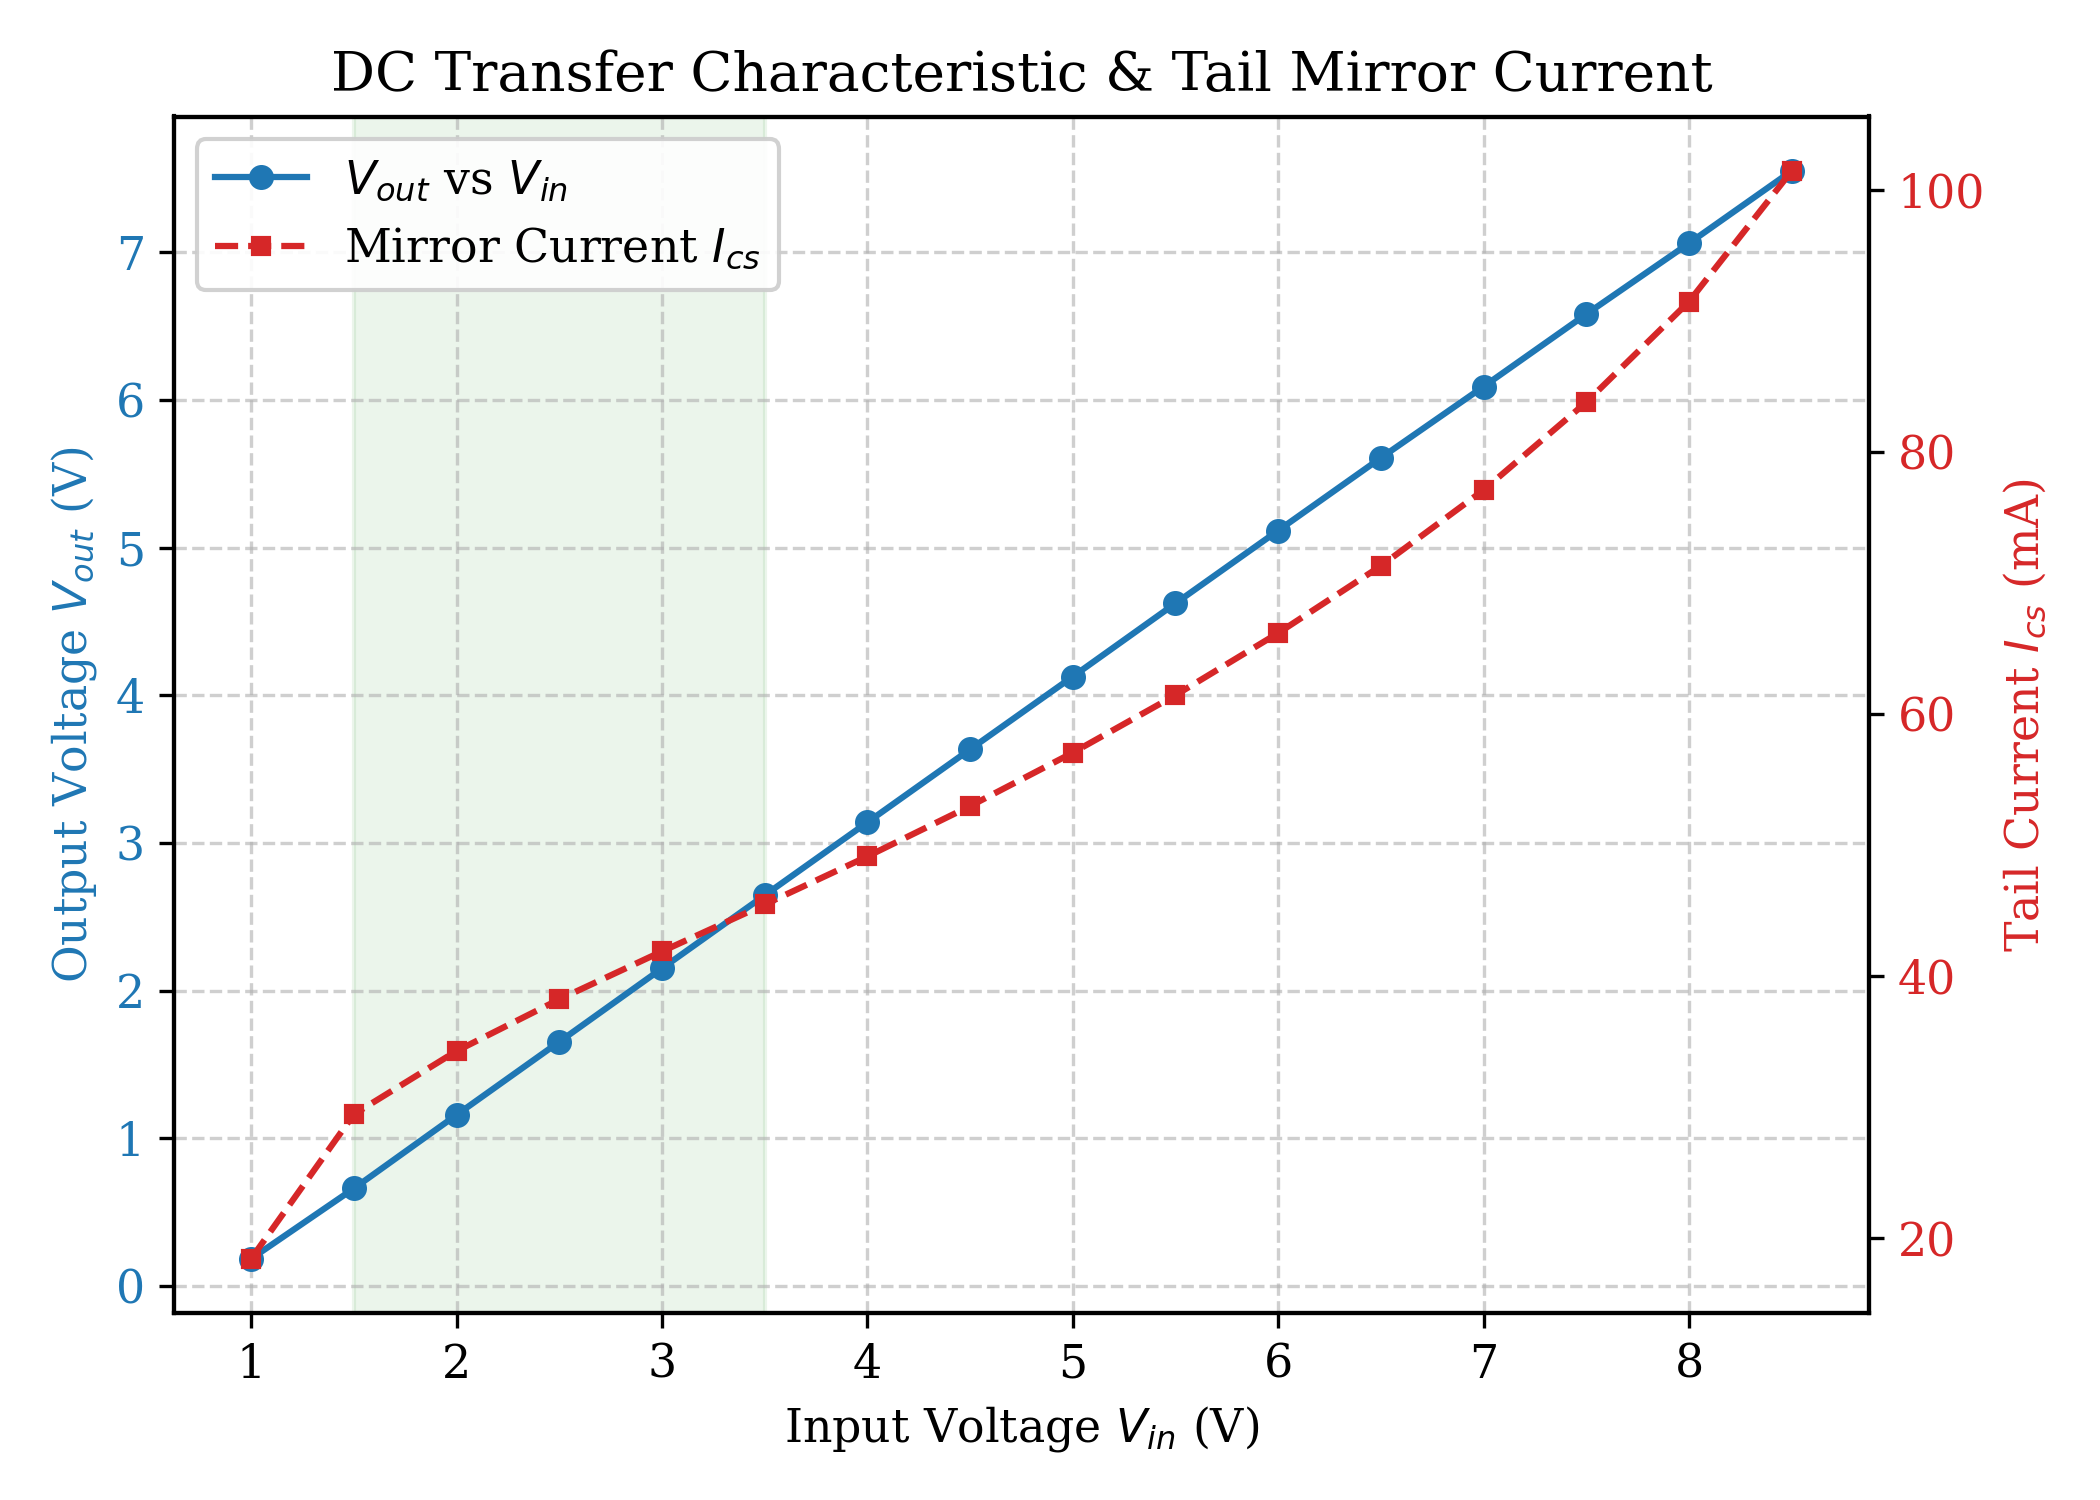
\includegraphics[width=\linewidth]{dc_transfer.png}
        \caption{Measured $V_{out}$ and Tail Current $I_{cs}$ vs.\ $V_{in}$.}
        \label{fig:dc_measured}
    \end{minipage}\hfill
    \begin{minipage}{0.48\textwidth}
        \centering
        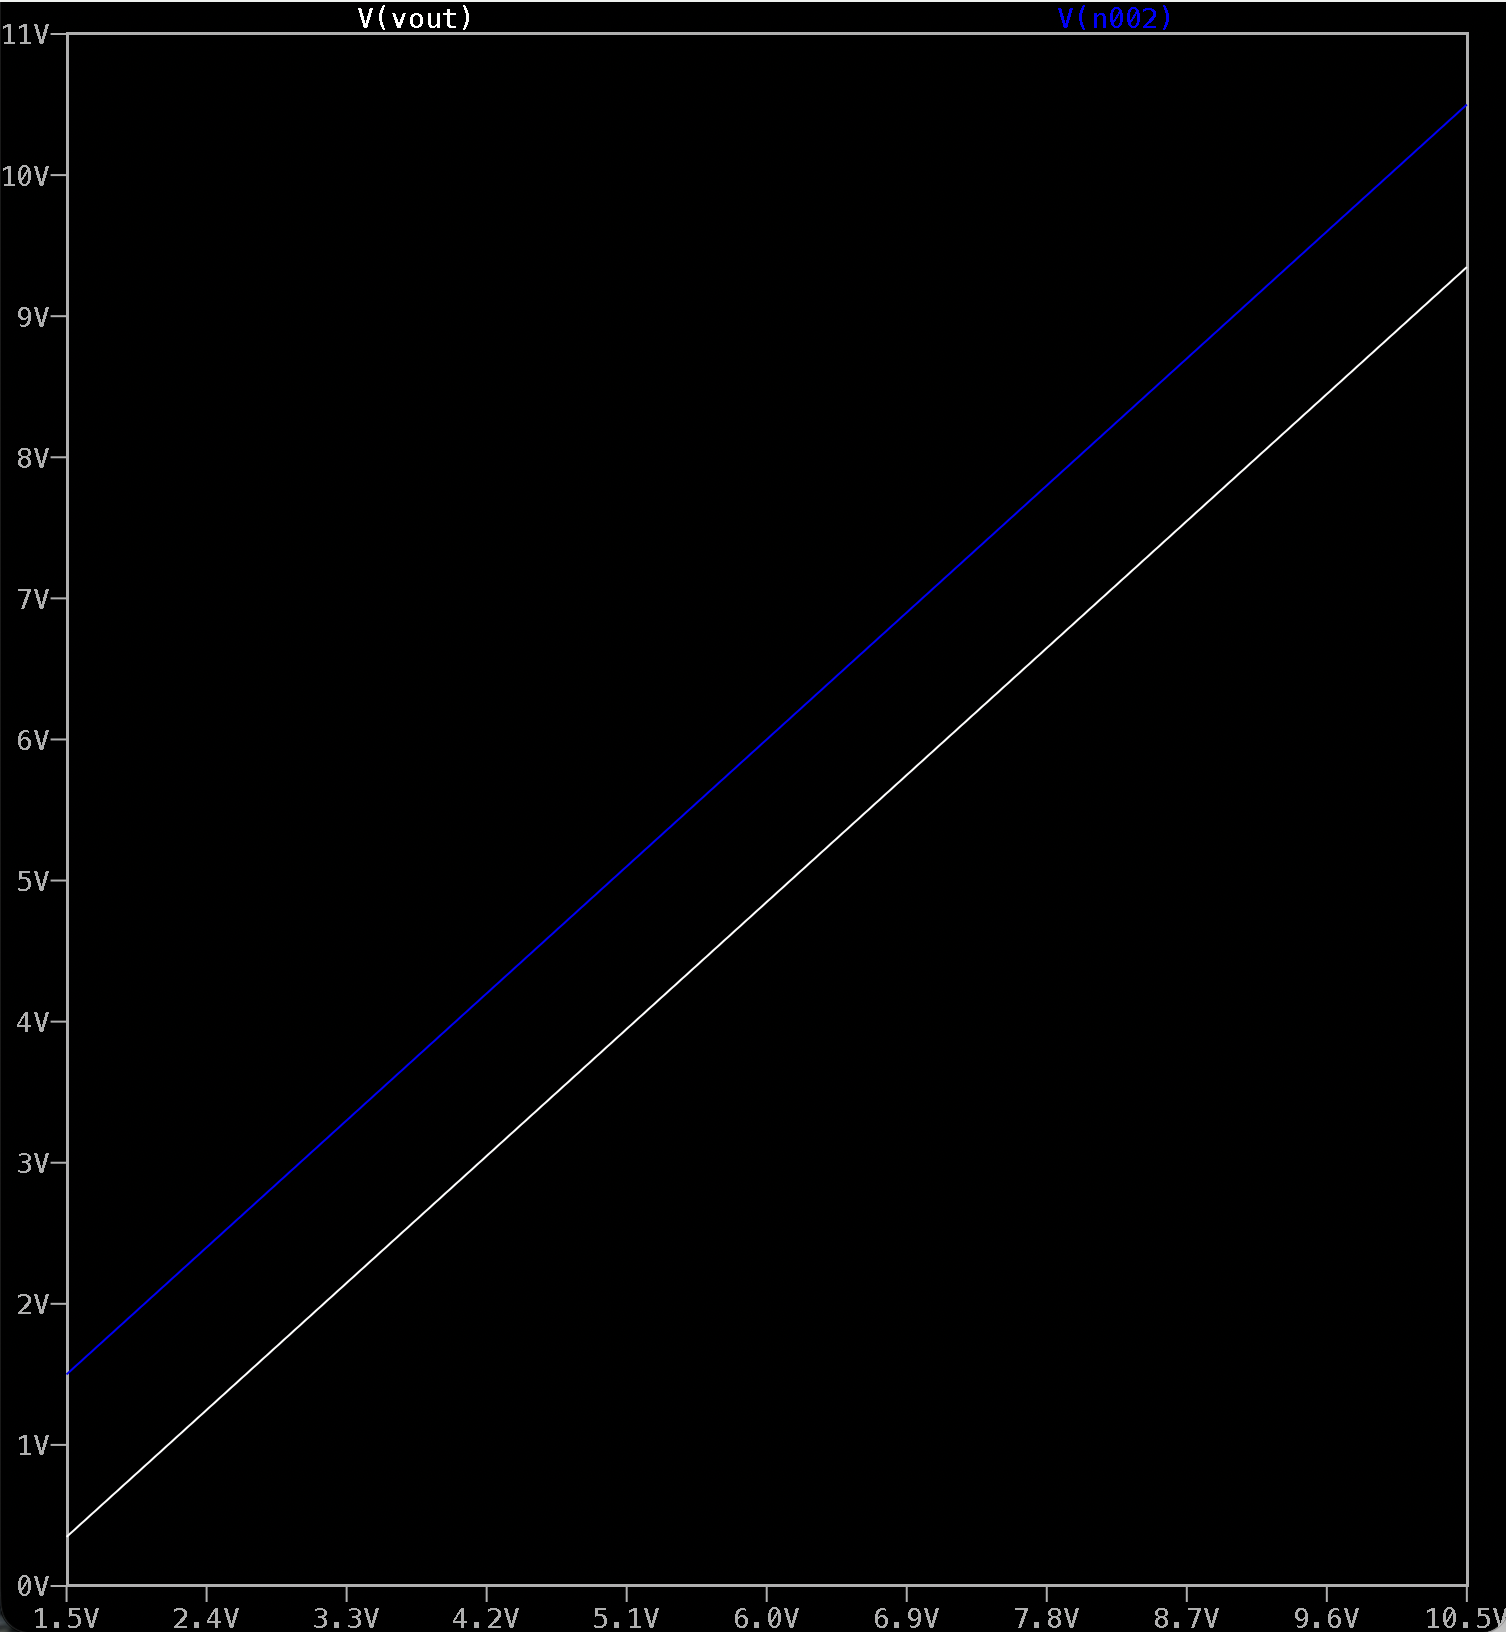
\includegraphics[width=\linewidth]{simulation_dc.png}
        \caption{LTspice Simulated DC Transfer Curve ($V_{in}$ swept 1.5~V to 10.5~V).}
        \label{fig:dc_sim}
    \end{minipage}
\end{figure}

\noindent\textbf{Physical Analysis of Operating Regions:}
\begin{itemize}
    \item \textbf{Triode Boundary ($V_{in} < 1.5\text{ V}$):} At $V_{in} = 1.0\text{ V}$, $V_{out}$ is only $0.184\text{ V}$. Because the drain-source voltage of the mirror transistor is $V_{DS2} = V_{out} = 0.184\text{ V}$, $M_2$ falls out of saturation into the triode region ($V_{DS2} < V_{GS2} - V_{th}$), causing the tail current to collapse to $18.45\text{ mA}$.
    \item \textbf{Linear Saturation Region ($1.5\text{ V} \le V_{in} \le 3.5\text{ V}$):} In this valid window, both transistors remain saturated. The measured transfer slope is $\Delta V_{out} / \Delta V_{in} = 0.990\text{ V/V}$ with an average level shift of $0.847\text{ V}$, and the tail current sits reliably at its designed bias ($41.9\text{ mA}$ at $V_{in} = 3.0\text{ V}$).
    \item \textbf{Thermal Runaway ($V_{in} > 3.5\text{ V}$):} Above $3.5\text{ V}$, $V_{out}$ rises toward $7.55\text{ V}$. This subjects $M_2$ to high voltage and high current simultaneously ($V_{DS2} = 7.55\text{ V}$), dissipating $P = V_{DS2} \cdot I_{cs} \approx 0.77\text{ W}$ in the tiny uncooled SO-8 package. The resulting die heating lowers the MOSFET threshold voltage, driving tail current exponentially upward to $101.45\text{ mA}$.
\end{itemize}

\subsection{Small-Signal AC Frequency Response (Table 2)}
Holding the DC operating bias at $V_{in,DC} = 3.0\text{ V}$ ($I_{cs} = 41.9\text{ mA}$), an input sine wave of $200\text{ mV}_{p-p}$ was applied. The measured response across frequency is recorded in Table~\ref{tab:ac_data}.

\begin{table}[H]
    \centering
    \begin{tabular}{cccc}
        \toprule
        \textbf{Frequency (Hz)} & \textbf{$V_{out}$ Amplitude ($mV_{p-p}$)} & \textbf{Gain $|A_v|$ (V/V)} & \textbf{Gain (dB)} \\
        \midrule
        6      & 192 & 0.960 & -0.35 \\
        8      & 192 & 0.960 & -0.35 \\
        10     & 192 & 0.960 & -0.35 \\
        30     & 194 & 0.970 & -0.26 \\
        100    & 194 & 0.970 & -0.26 \\
        300    & 194 & 0.970 & -0.26 \\
        1000   & 196 & 0.980 & -0.18 \\
        3000   & 196 & 0.980 & -0.18 \\
        10000  & 198 & 0.990 & -0.09 \\
        30000  & 200 & 1.000 & \phantom{-}0.00 \\
        100000 & 200 & 1.000 & \phantom{-}0.00 \\
        \bottomrule
    \end{tabular}
    \caption{Measured AC Frequency Response from 6~Hz to 100~kHz ($V_{in} = 200\text{ mV}_{p-p}$)}
    \label{tab:ac_data}
\end{table}

\begin{figure}[H]
    \centering
    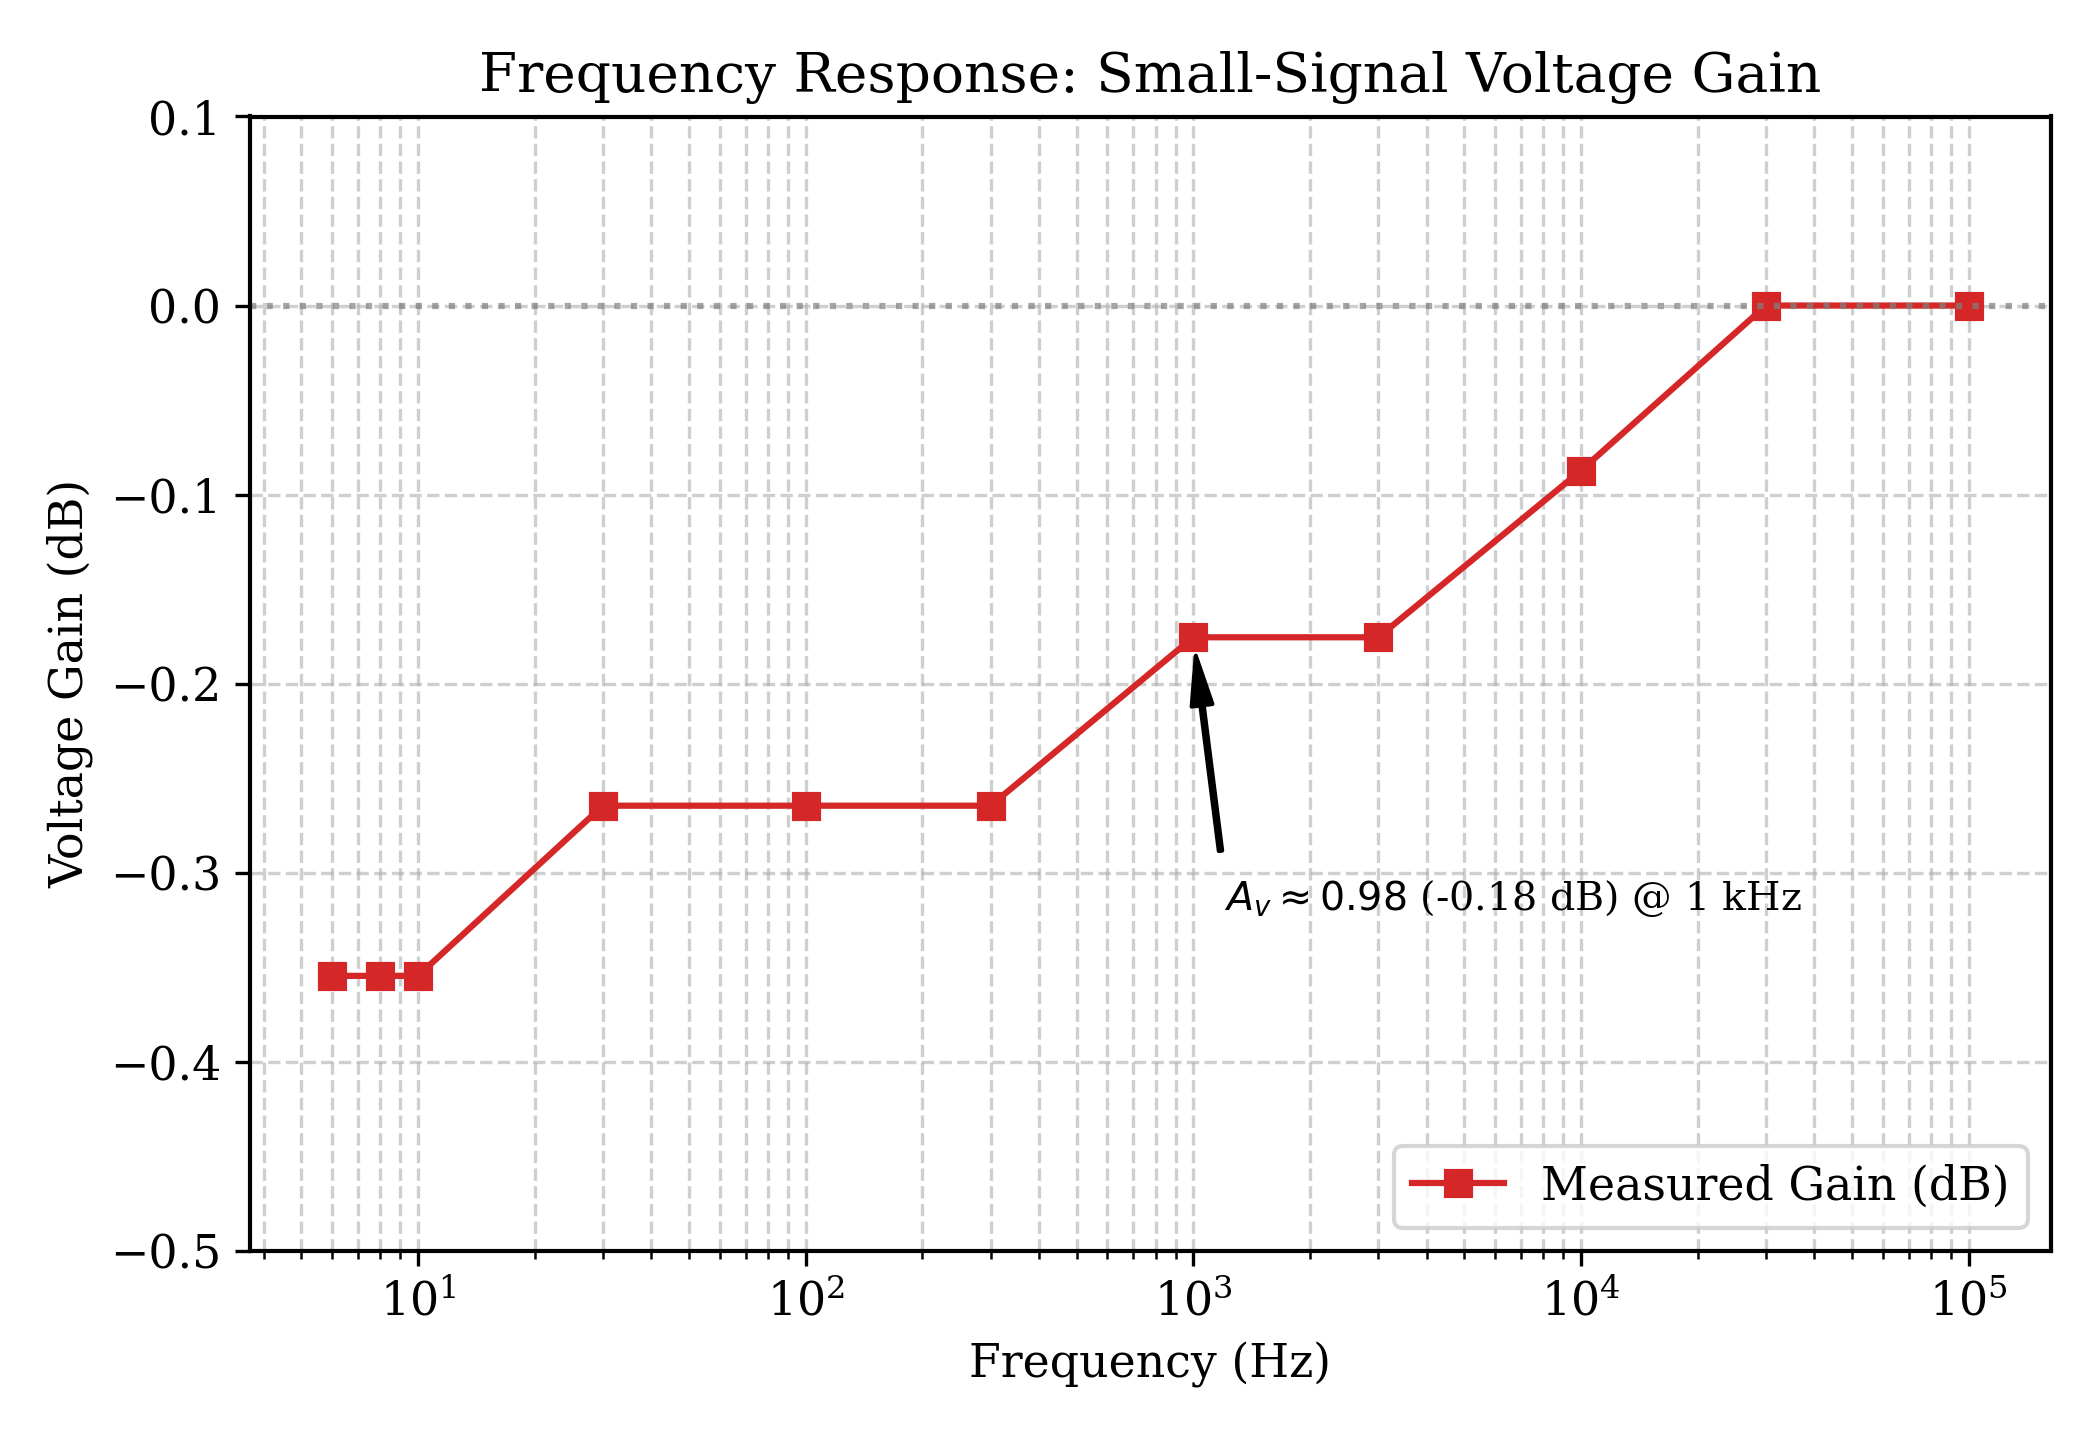
\includegraphics[width=0.6\textwidth]{bode_plot.png}
    \caption{Measured Bode Plot: Small-Signal Voltage Gain vs.\ Frequency.}
    \label{fig:bode}
\end{figure}

As shown in Figure~\ref{fig:bode}, the frequency response is virtually flat across the entire four-decade span. At the reference frequency of 1~kHz, the measured gain is $|A_v| = 0.980\text{ V/V}$ ($-0.18\text{ dB}$). There is no high-frequency roll-off up to 100~kHz.

\subsection{Output Resistance Loading Measurements (Table 3)}
Table~\ref{tab:rout_data} presents the output loading data at 1~kHz alongside the theoretical loading ratios predicted for our $V_{DD} = 10\text{ V}$ experimental setup ($\text{Ratio}_{pred} = R_L / (R_L + 1.18\ \Omega)$) and the lab manual's nominal $12\text{ V}$ specification ($\text{Ratio}_{manual} = R_L / (R_L + 0.96\ \Omega)$).

\begin{table}[H]
    \centering
    \small
    \setlength{\tabcolsep}{3.5pt}
    \begin{tabular}{ccccc}
        \toprule
        \textbf{$R_L$ ($\Omega$)} & \textbf{$V_{out}$ Loaded ($mV_{p-p}$)} & \textbf{Measured Ratio} & \textbf{Pred. (10V)} & \textbf{Extracted $R_{out}$ ($\Omega$)} \\
        \midrule
        -- (unloaded) & 196.0 & 1.000 & 1.000 & -- \\
        10.2          & 174.0 & 0.888 & 0.896 & 1.29 \\
        47.0          & 188.0 & 0.959 & 0.975 & 2.00 \\
        112.0         & 192.0 & 0.980 & 0.990 & 2.33 \\
        \bottomrule
    \end{tabular}
    \caption{Output Resistance Loading Measurements at 1~kHz (compared with 10~V model $R_{out} \approx 1.18\ \Omega$).}
    \label{tab:rout_data}
\end{table}

\begin{figure}[H]
    \centering
    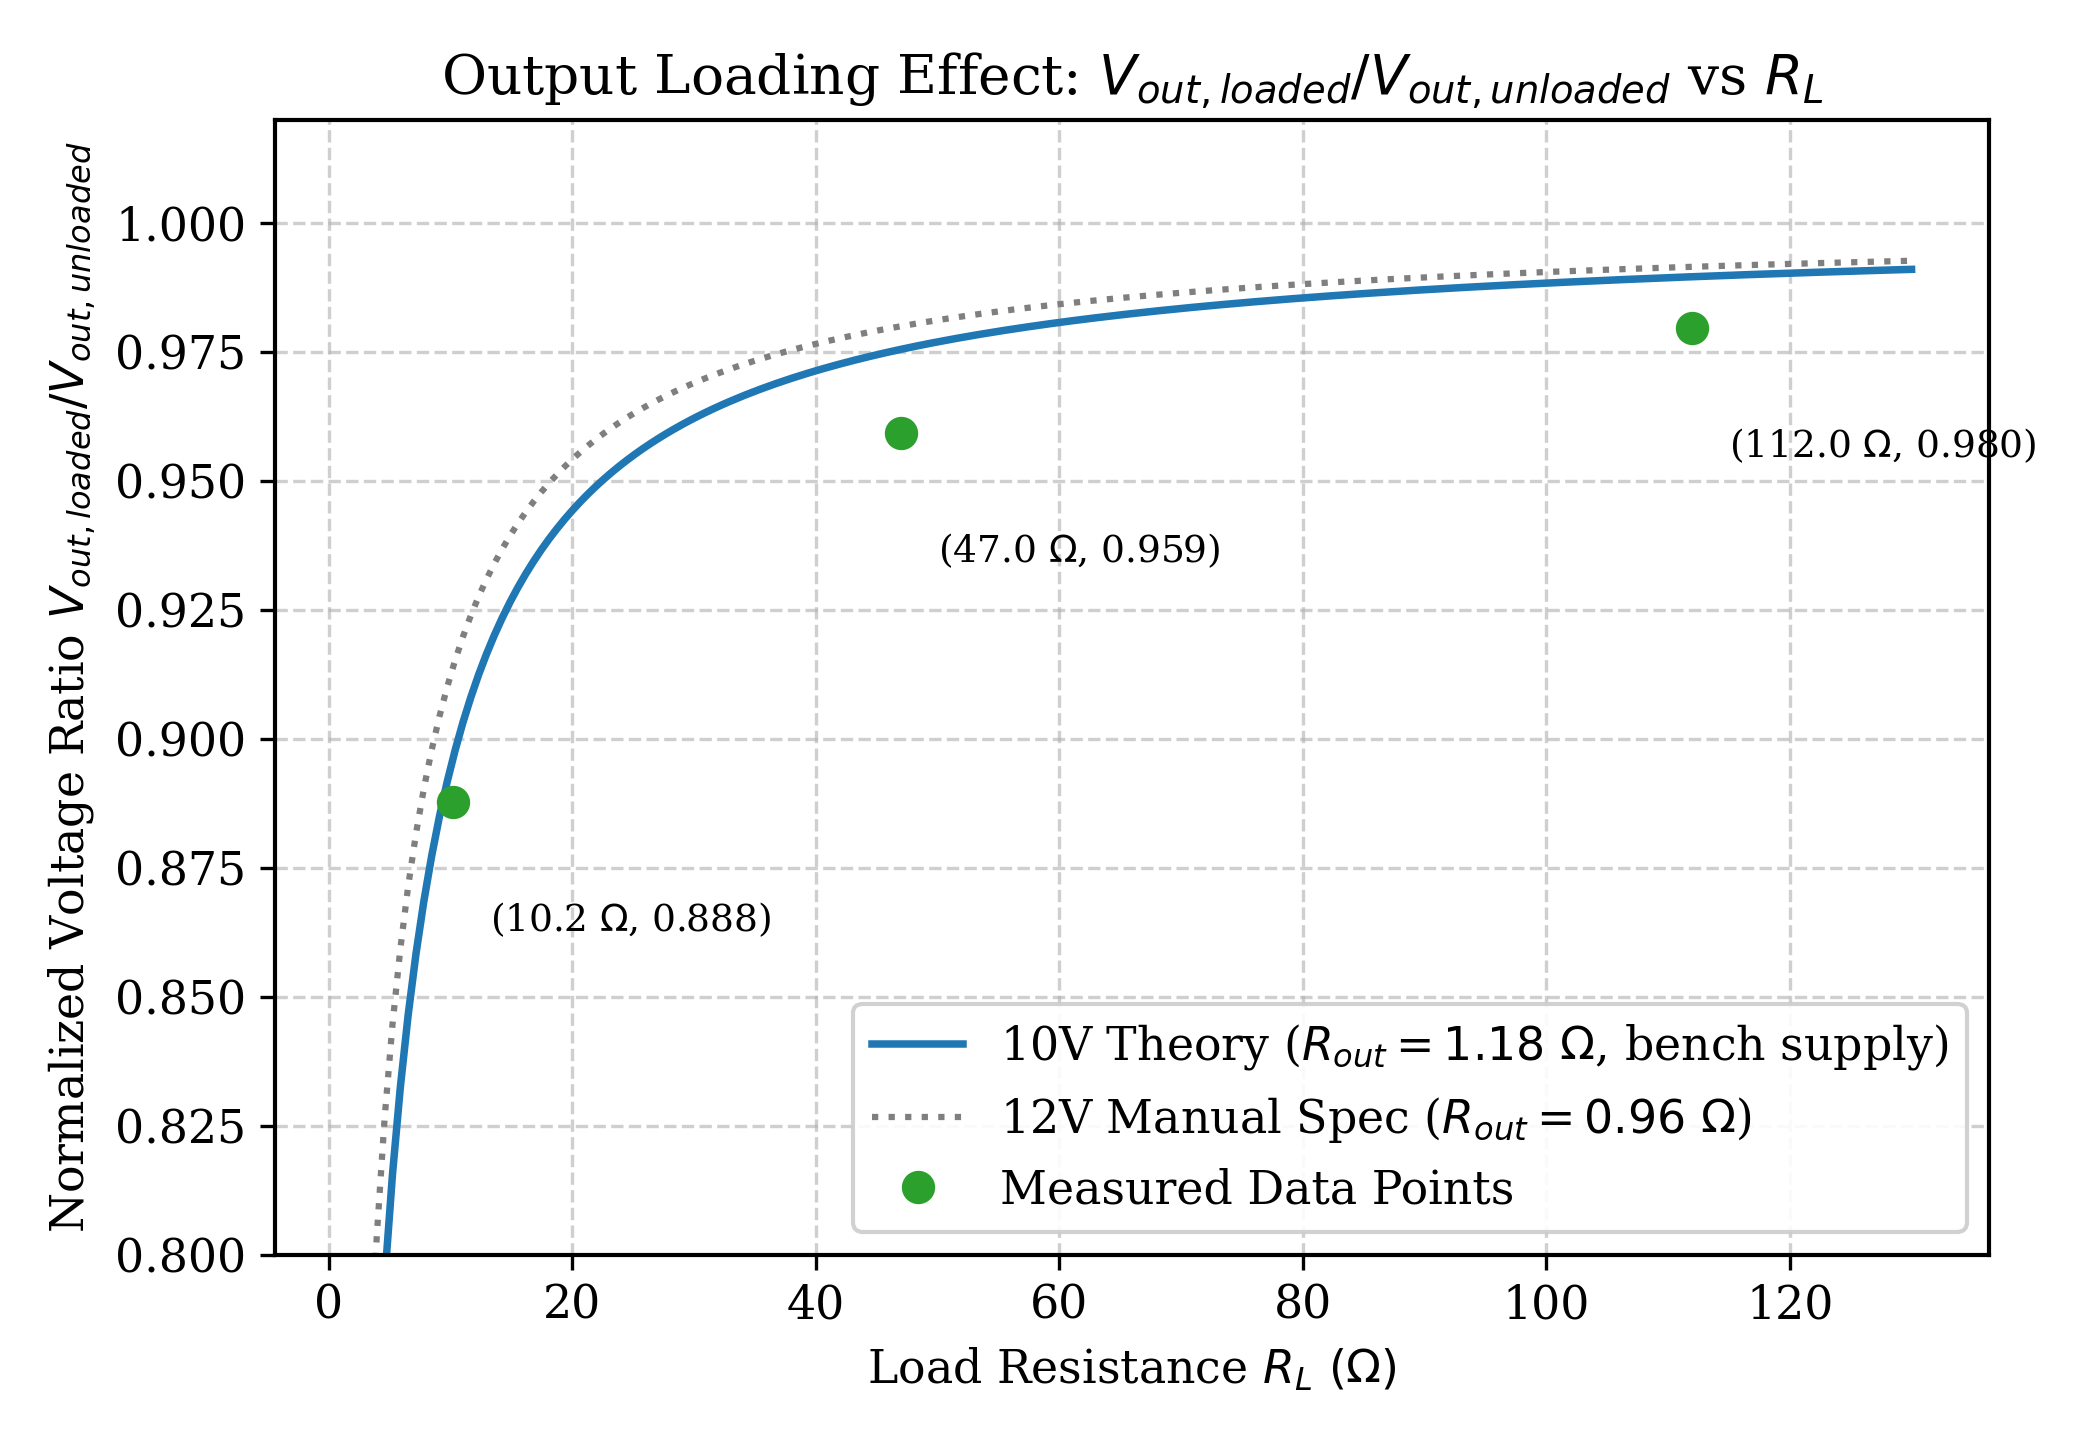
\includegraphics[width=0.48\textwidth]{loading_effect.png}
    \caption{Normalized Output Voltage Ratio vs.\ Load Resistance $R_L$ overlaid with 10~V Theoretical Model ($R_{out} = 1.18\ \Omega$) and 12~V Manual Specification ($R_{out} = 0.96\ \Omega$).}
    \label{fig:loading}
\end{figure}

Using the voltage divider formula $R_{out} = R_L \left(\frac{V_{out,unloaded}}{V_{out,loaded}} - 1\right)$, the extracted output resistances are $1.29\ \Omega$, $2.00\ \Omega$, and $2.33\ \Omega$.

\section{Calculations and Verification}

\subsection{Linear DC Slope and Level Shift}
Using the stable linear region between $V_{in} = 3.0\text{ V}$ and $3.5\text{ V}$:
\begin{equation}
\text{DC Slope } \frac{\Delta V_{out}}{\Delta V_{in}} = \frac{2.645\text{ V} - 2.150\text{ V}}{3.5\text{ V} - 3.0\text{ V}} = \frac{0.495\text{ V}}{0.500\text{ V}} = 0.990\text{ V/V}
\end{equation}
Averaging the level shift across the linear operating region ($1.5\text{ V}$ to $3.5\text{ V}$):
\begin{equation}
V_{shift,avg} = \frac{0.840 + 0.842 + 0.847 + 0.850 + 0.855}{5} = 0.847\text{ V}
\end{equation}

\subsection{Small-Signal Gain and LTspice Transient Verification}
At the 1~kHz test frequency, the measured small-signal voltage gain is:
\begin{equation}
A_v(1\text{ kHz}) = \frac{196\text{ mV}}{200\text{ mV}} = 0.980\text{ V/V} \quad (-0.18\text{ dB})
\end{equation}
To verify the AC operating point and small-signal tracking, the circuit was simulated in LTspice using the schematic in Figure~\ref{fig:sim_ac}(a) ($V_{DD} = 10\text{ V}$, $V_{bias} = 3\text{ V}$, $C_{in} = 1\ \mu\text{F}$, $R_{bias} = 1\text{ M}\Omega$, $200\text{ mV}_{p-p}$ sine at 1~kHz). The resulting transient waveforms in Figure~\ref{fig:sim_ac}(b) confirm near-ideal follower behavior: a $200\text{ mV}_{p-p}$ input produces an identical $200\text{ mV}_{p-p}$ output sinusoid with $A_v \approx 1.00\text{ V/V}$.

\begin{figure}[H]
    \centering
    \begin{minipage}{0.53\textwidth}
        \centering
        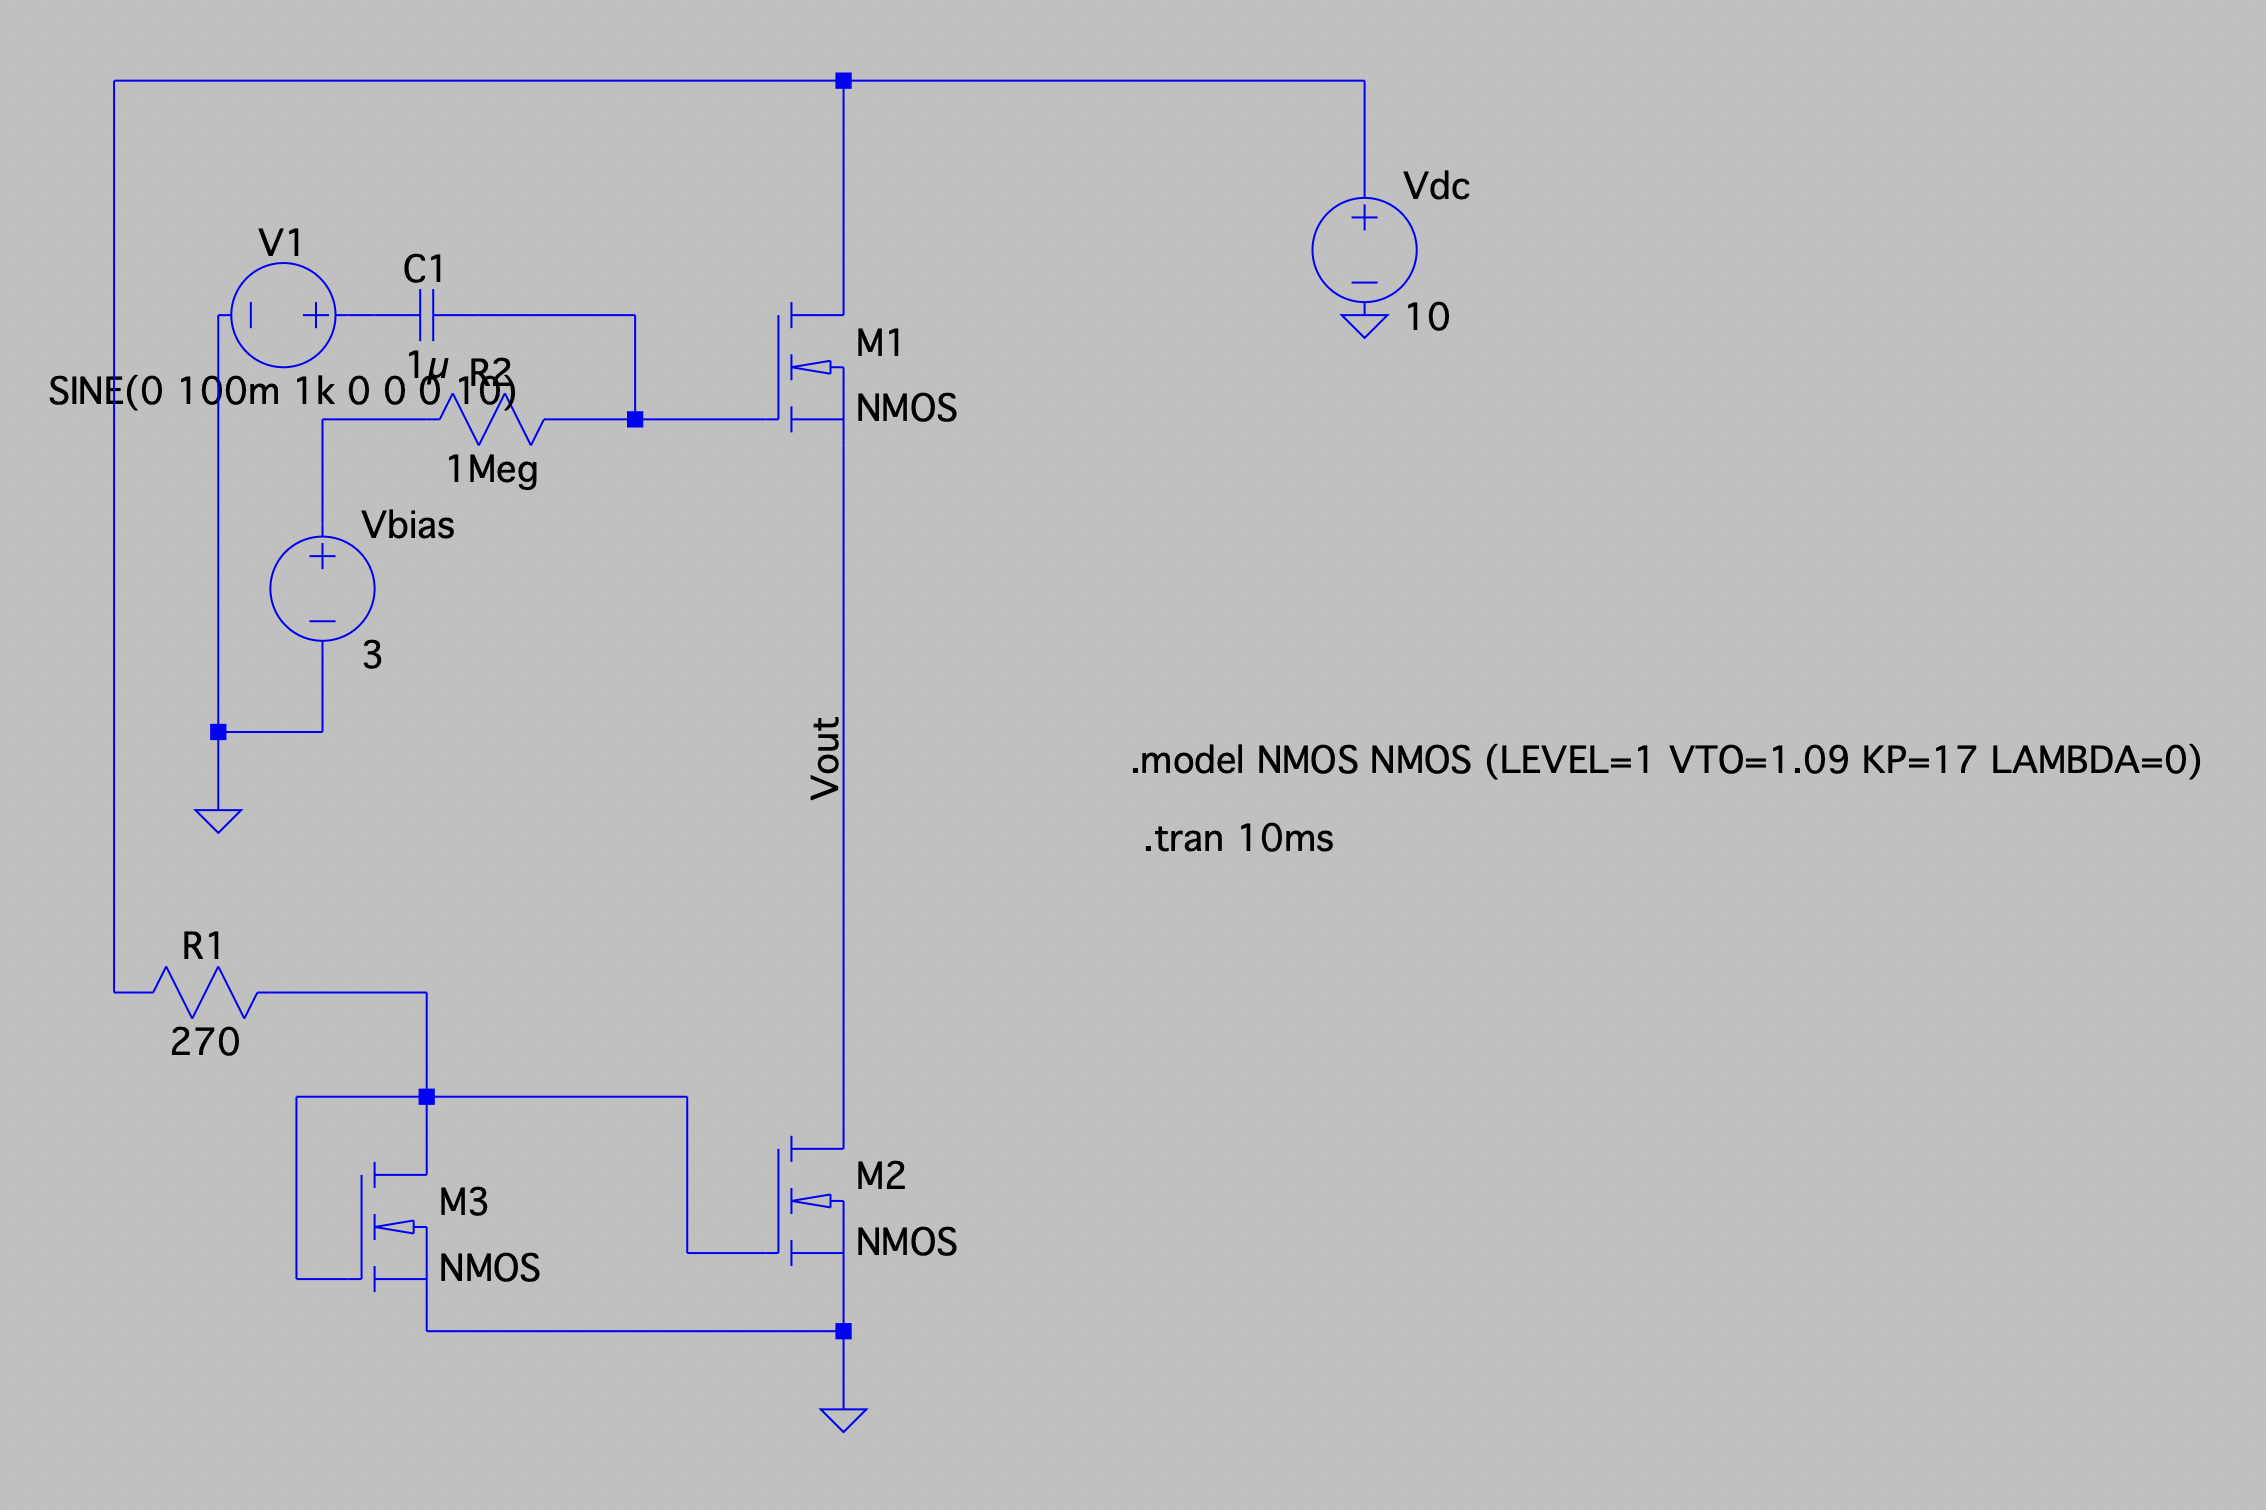
\includegraphics[height=2.0cm]{ckt_ac.png}
        \caption*{(a) AC Simulation Schematic ($V_{bias}=3\text{ V}$)}
    \end{minipage}\hfill
    \begin{minipage}{0.45\textwidth}
        \centering
        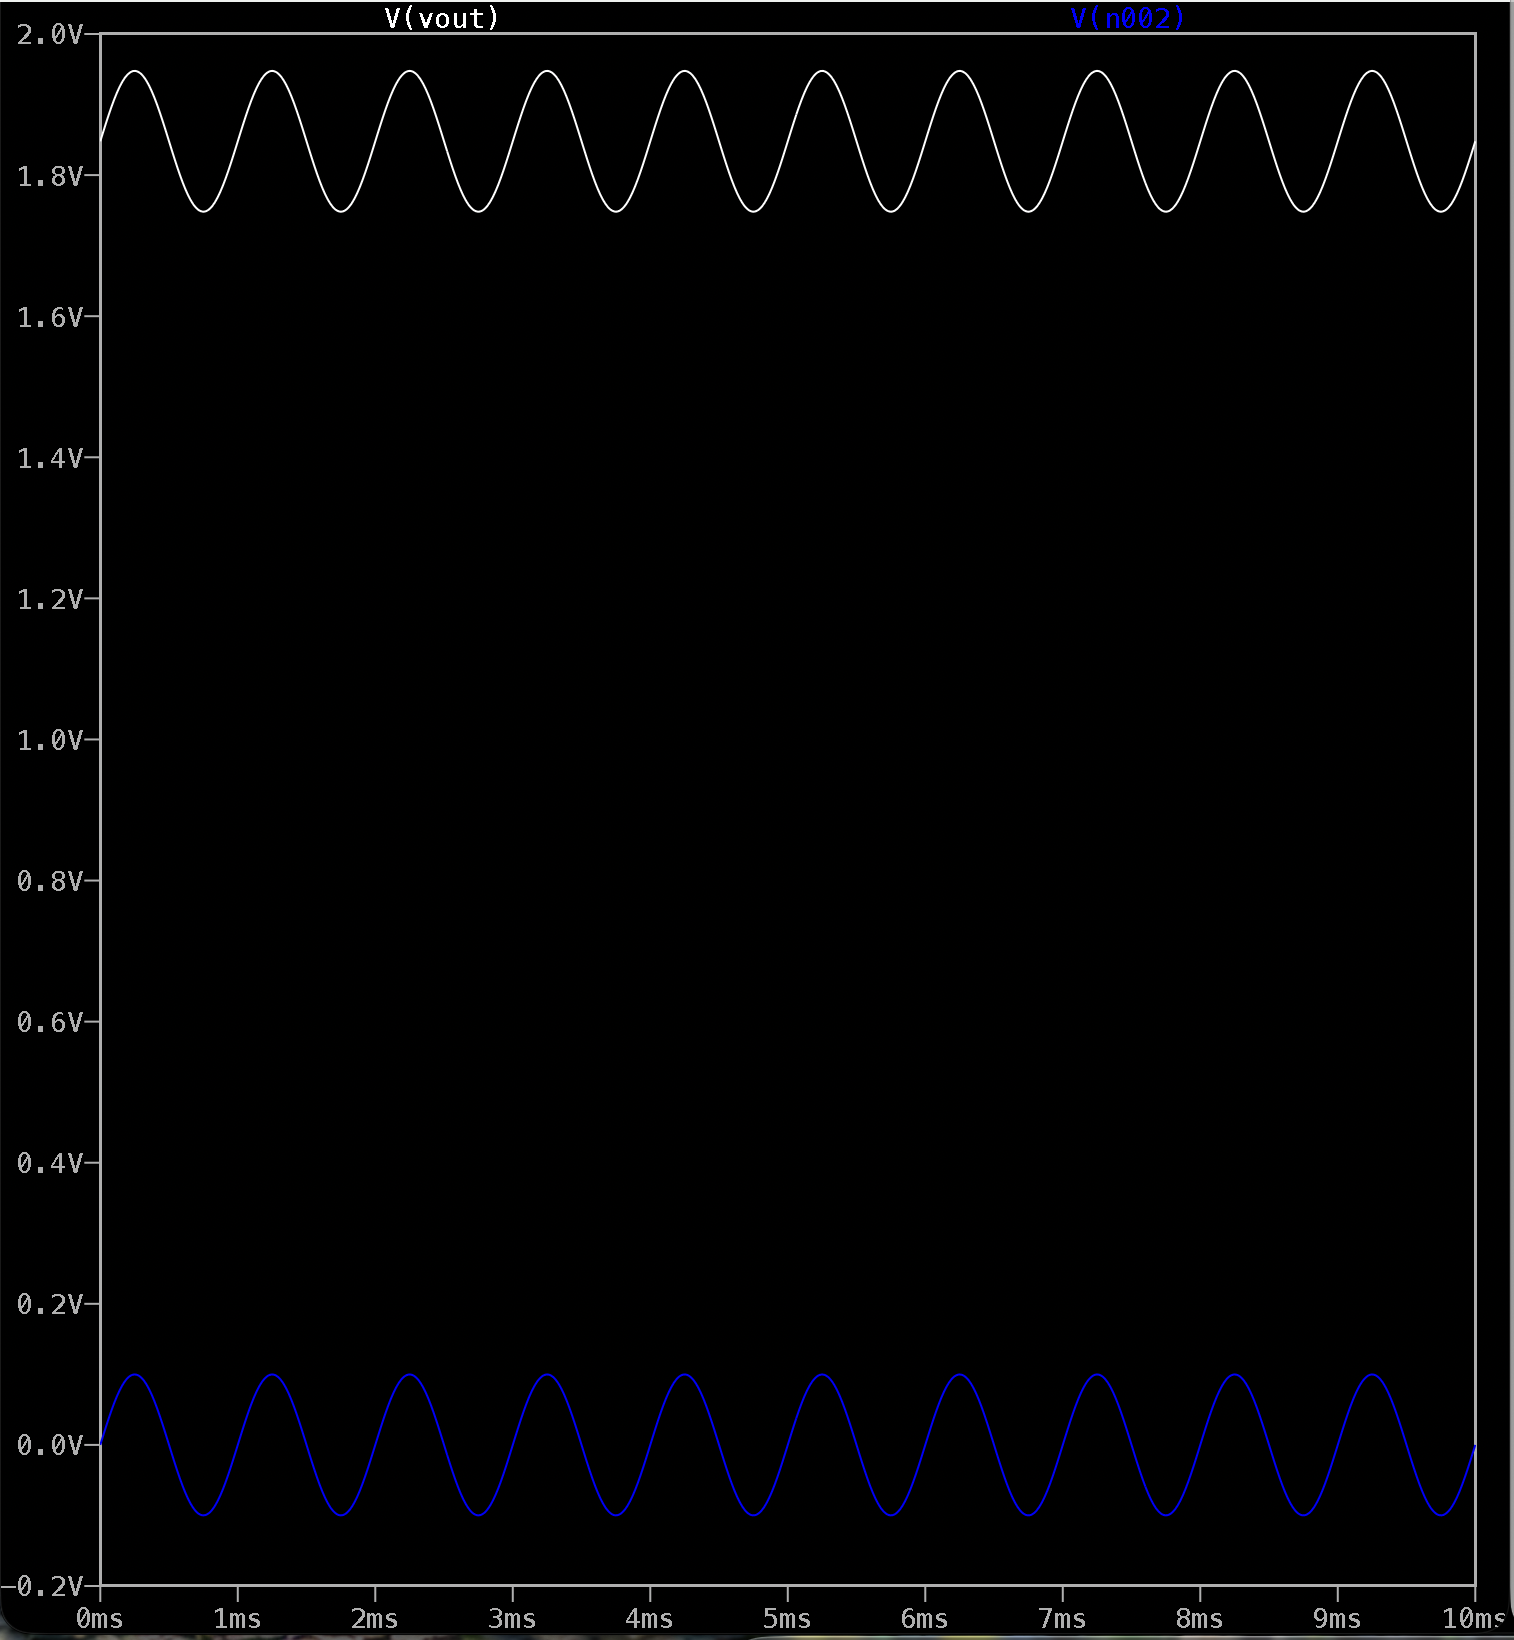
\includegraphics[height=2.0cm]{simulation_ac_1kHz.png}
        \caption*{(b) 1~kHz Transient Output ($A_v \approx 1.00$)}
    \end{minipage}
    \vspace{-2ex}
    \caption{LTspice AC Simulation Setup and 1~kHz Transient Verification: (a) Schematic showing input coupling network ($C_{in} = 1\ \mu\text{F}$, $R_{bias} = 1\text{ M}\Omega$) and (b) simulated transient waveforms confirming unity-gain tracking.}
    \label{fig:sim_ac}
\end{figure}
\vspace{-1.5ex}

\subsection{Bandwidth Evaluation and Theoretical Summary Comparison}
Per Section~10 of the laboratory manual, the AC frequency response from Table~\ref{tab:ac_data} was evaluated for roll-off behavior. Across 10~kHz, 30~kHz, and 100~kHz, the measured gain remained flat at $0.990\text{--}1.000\text{ V/V}$ ($0.00\text{ dB}$) with zero observable high-frequency roll-off. This substantiates Section~4: because $R_{out} \approx 1.87\ \Omega$ is remarkably small, the output pole $f_{p,out} = \frac{1}{2\pi R_{out} C_{out}}$ sits above several tens of megahertz, ensuring bandwidth within the sweep band is unconstrained by the active follower. At the lowest frequencies (6--10~Hz), output amplitude dipped marginally to $192\text{ mV}_{p-p}$ ($|A_v| = 0.960\text{ V/V}$, $-0.35\text{ dB}$) due entirely to the high-pass input coupling network ($C_{in} = 1\ \mu\text{F}$, $R_{bias} = 1\text{ M}\Omega$) rather than any limitation of the transistor stage.

Averaging the three extracted values from Table~\ref{tab:rout_data} yields $R_{out,measured} = \frac{1.29 + 2.00 + 2.33}{3} \approx 1.87\ \Omega$. Following Section~10 of the manual, the comparison between theoretical predictions and measured results is summarized in Table~\ref{tab:comparison}.

\begin{table}[H]
    \centering
    \small
    \vspace{-1ex}
    \begin{tabular}{lccc}
        \toprule
        \textbf{Quantity} & \textbf{Predicted} & \textbf{Measured} & \textbf{\% Deviation} \\
        \midrule
        DC slope $\Delta V_{out} / \Delta V_{in}$ & 1.00 & 0.990 & 1.0\% \\
        Level shift $V_{in} - V_{out}$ (V)    & 1.09 & 0.847 & 22.3\% \\
        Small-signal $A_v$ (1 kHz)               & 1.00 & 0.980 & 2.0\% \\
        Output resistance $R_{out}$ (10V theory) & 1.18~$\Omega$ & 1.87~$\Omega$ & 58.5\% \\
        Output resistance $R_{out}$ (12V manual) & 0.96~$\Omega$ & 1.87~$\Omega$ & 94.8\% \\
        \bottomrule
    \end{tabular}
    \vspace{-1ex}
    \caption{Summary Comparison of Theoretical Predictions and Measured Results (Section 10 Table).}
    \label{tab:comparison}
\end{table}
\vspace{-1ex}

\noindent\textbf{Discussion of Discrepancies:} Both DC slope and small-signal gain matched ideal predictions within 1--2\%, confirming high mirror output resistance and negligible body effect ($V_{SB}=0$). The 22.3\% level shift difference ($0.847\text{ V}$ vs $1.09\text{ V}$) is due to the factory threshold spread of the SI9926BDY ($V_{GS(th)} = 0.6\text{--}1.5\text{ V}$), our physical sample exhibiting $V_{GS} \approx 0.85\text{ V}$ at 40~mA. For output resistance, while the manual's nominal 12V calculation predicted $R_{out} \approx 0.96\ \Omega$, our $V_{DD} = 10\text{ V}$ experimental supply lowers the reference current to $I_{ref} \approx 33\text{ mA}$, yielding an adjusted theoretical prediction of $R_{out} \approx 1.18\ \Omega$. This reduces the deviation to 58.5\% (vs 94.8\%), with the remaining gap cleanly explained by breadboard and jumper contact resistance ($0.4\text{--}0.6\ \Omega$) and subthreshold ideality factor ($n \approx 1.7$).

\clearpage
\section{Oscilloscope Waveforms}
Oscilloscope captures of the input and output waveforms across the sweep frequencies are presented in Figures~8 through~15. Across all captured frequencies, the output cleanly tracks the sinusoidal input with near-unity amplitude and negligible phase distortion.

\begin{figure}[H]
    \centering
    \begin{minipage}{0.48\textwidth}
        \centering
        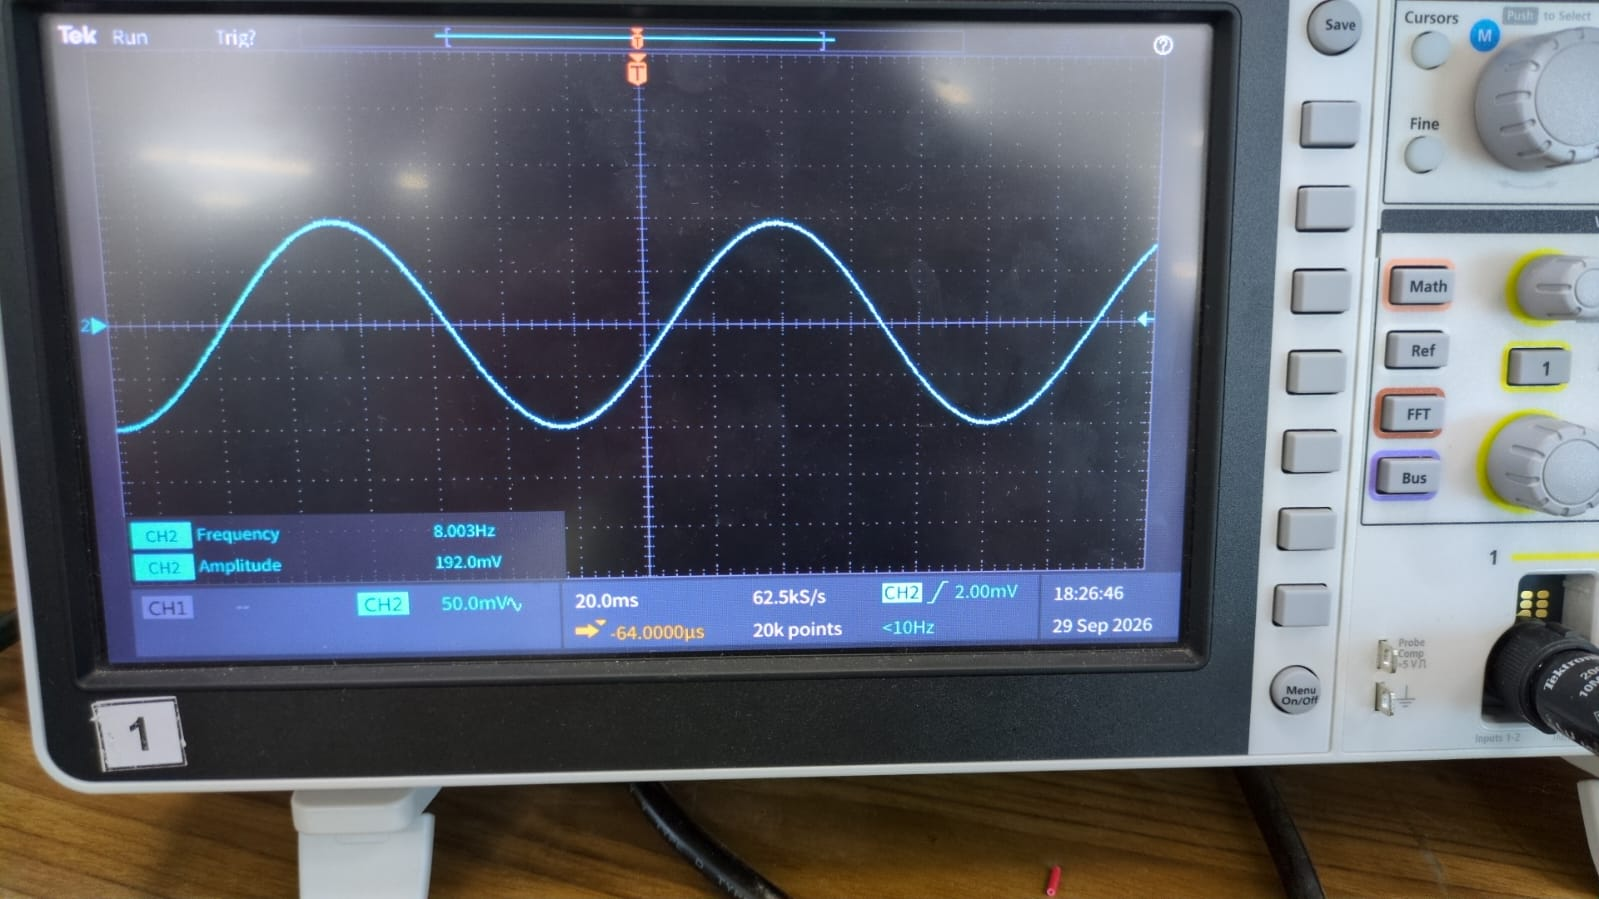
\includegraphics[height=2.5cm]{8Hz.jpeg}
        \caption{8~Hz Response.}
    \end{minipage}\hfill
    \begin{minipage}{0.48\textwidth}
        \centering
        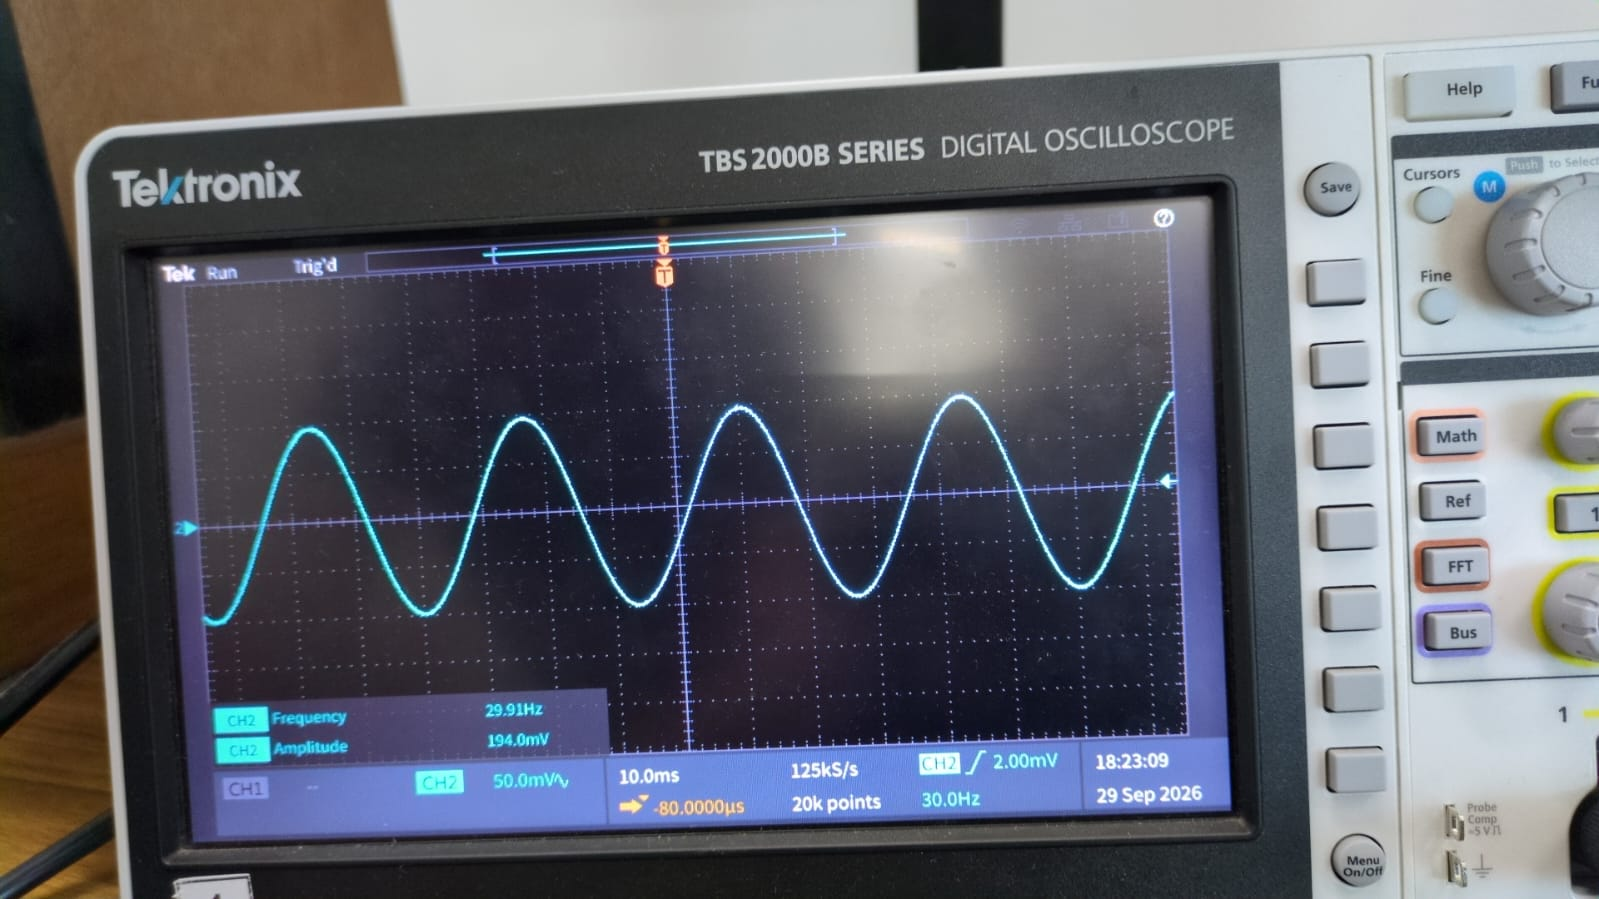
\includegraphics[height=2.5cm]{30Hz.jpeg}
        \caption{30~Hz Response.}
    \end{minipage}\\[0.4ex]
    \begin{minipage}{0.48\textwidth}
        \centering
        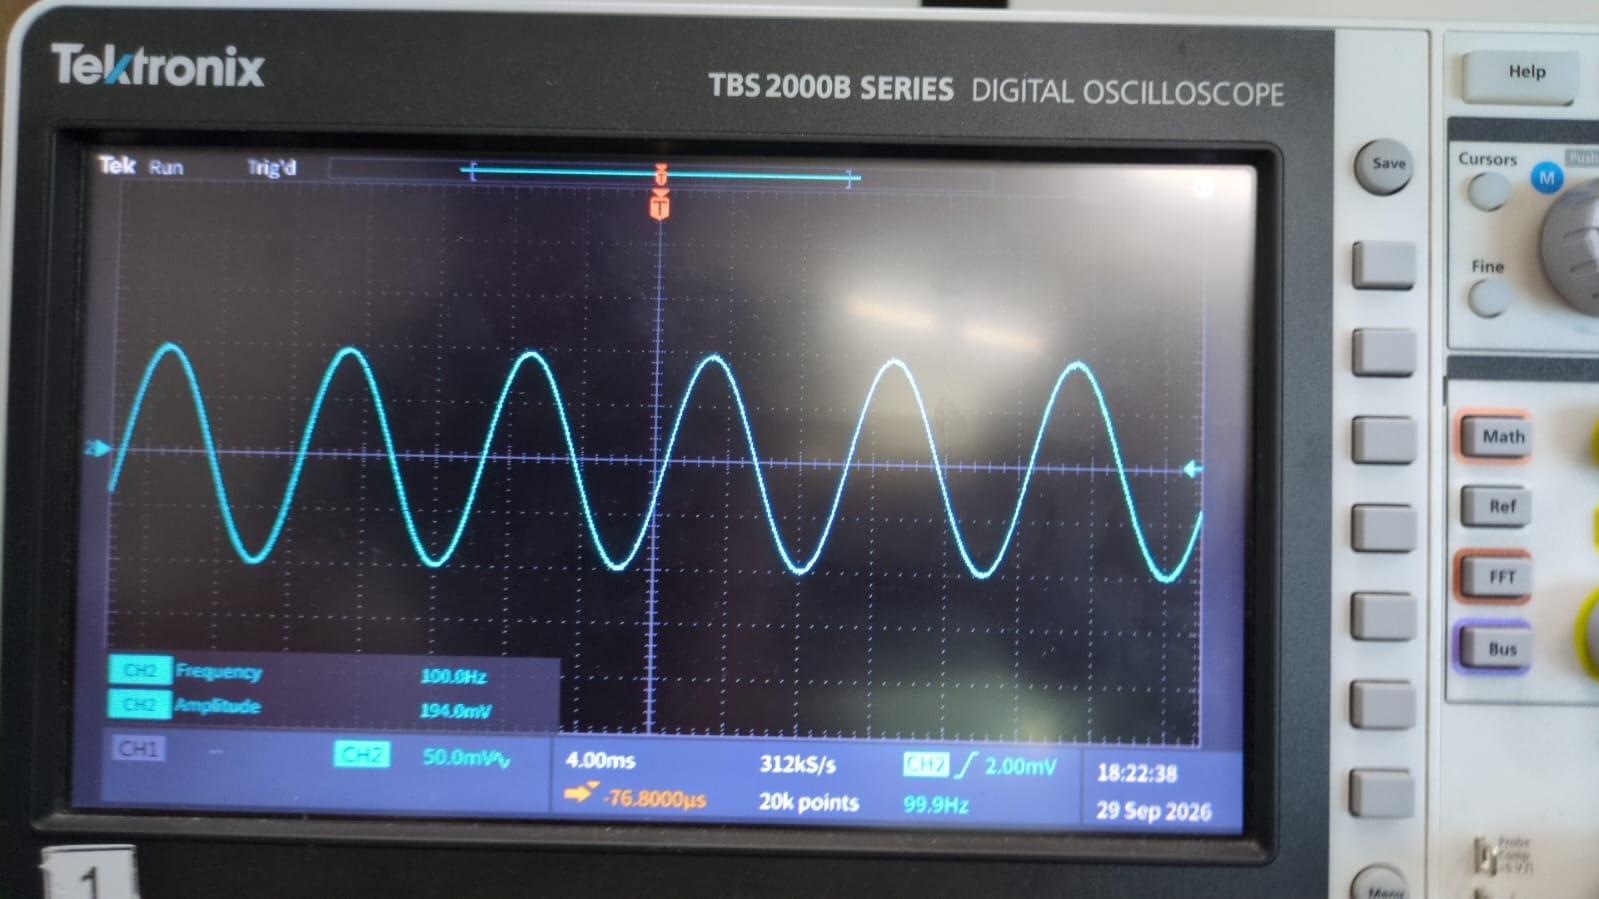
\includegraphics[height=2.5cm]{100Hz.jpeg}
        \caption{100~Hz Response.}
    \end{minipage}\hfill
    \begin{minipage}{0.48\textwidth}
        \centering
        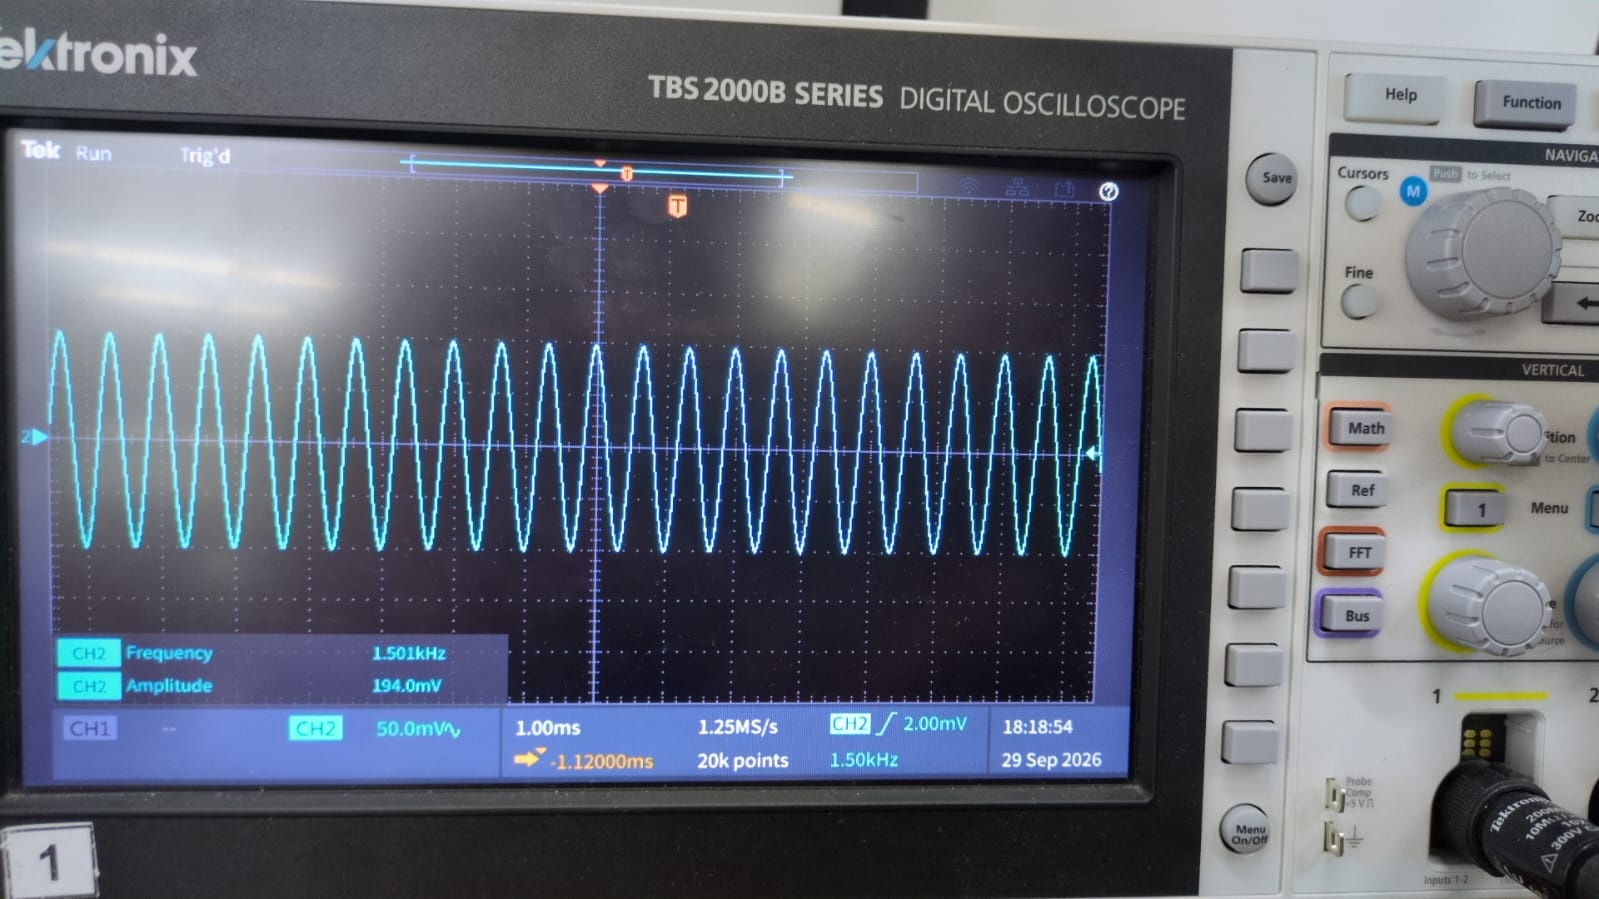
\includegraphics[height=2.5cm]{1.5kHz.jpeg}
        \caption{1.5~kHz Response.}
    \end{minipage}\\[0.4ex]
    \begin{minipage}{0.48\textwidth}
        \centering
        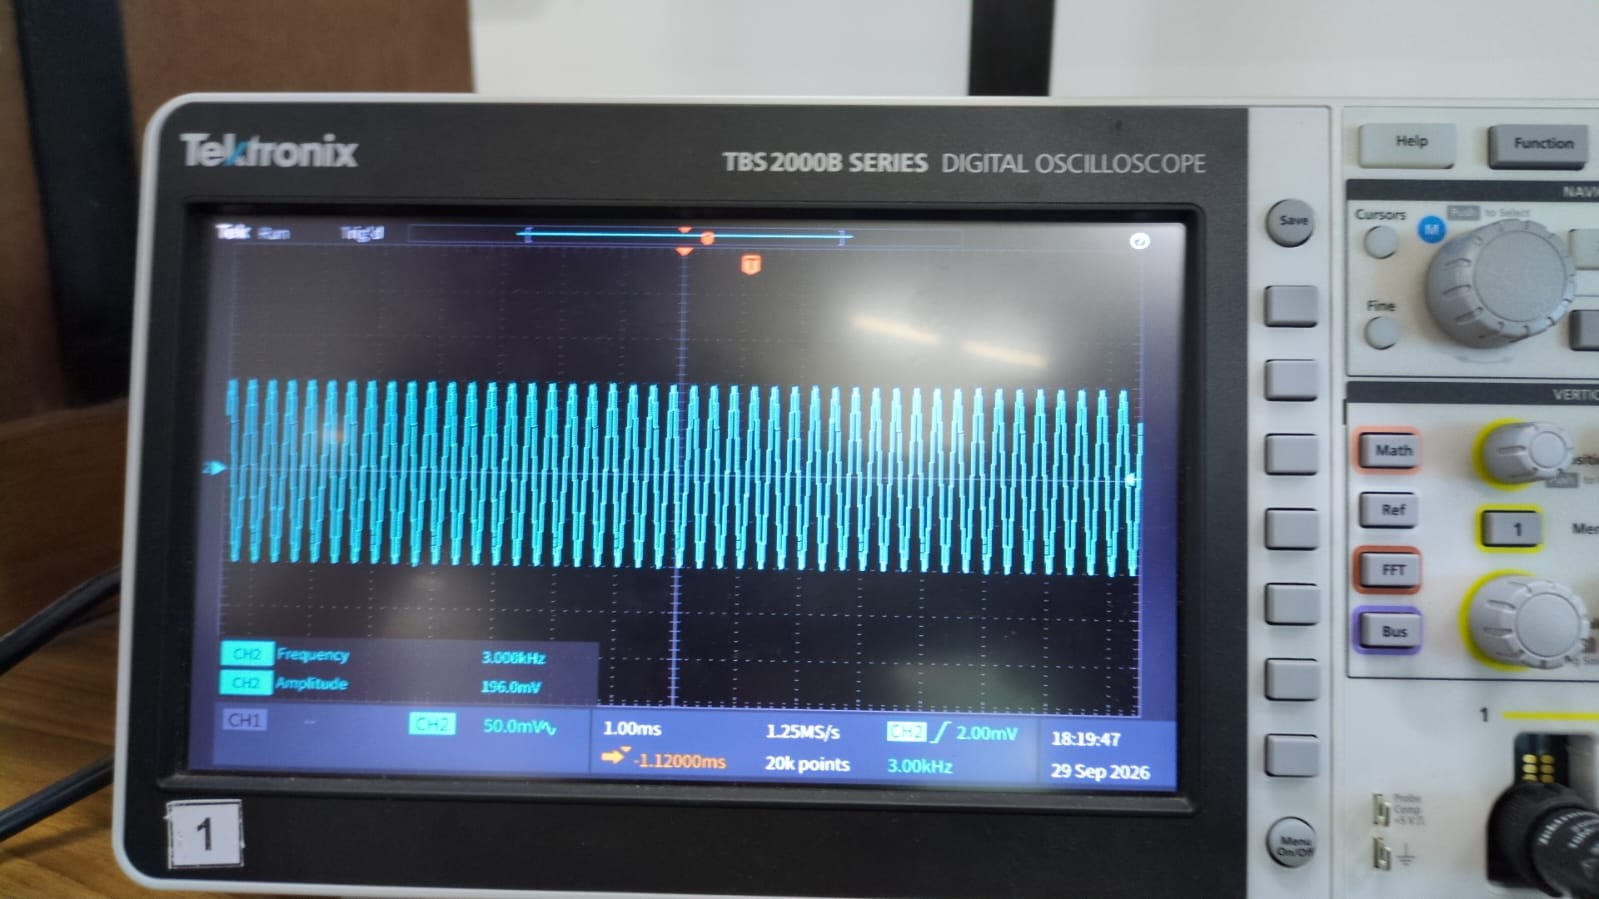
\includegraphics[height=2.5cm]{3kHz.jpeg}
        \caption{3~kHz Response.}
    \end{minipage}\hfill
    \begin{minipage}{0.48\textwidth}
        \centering
        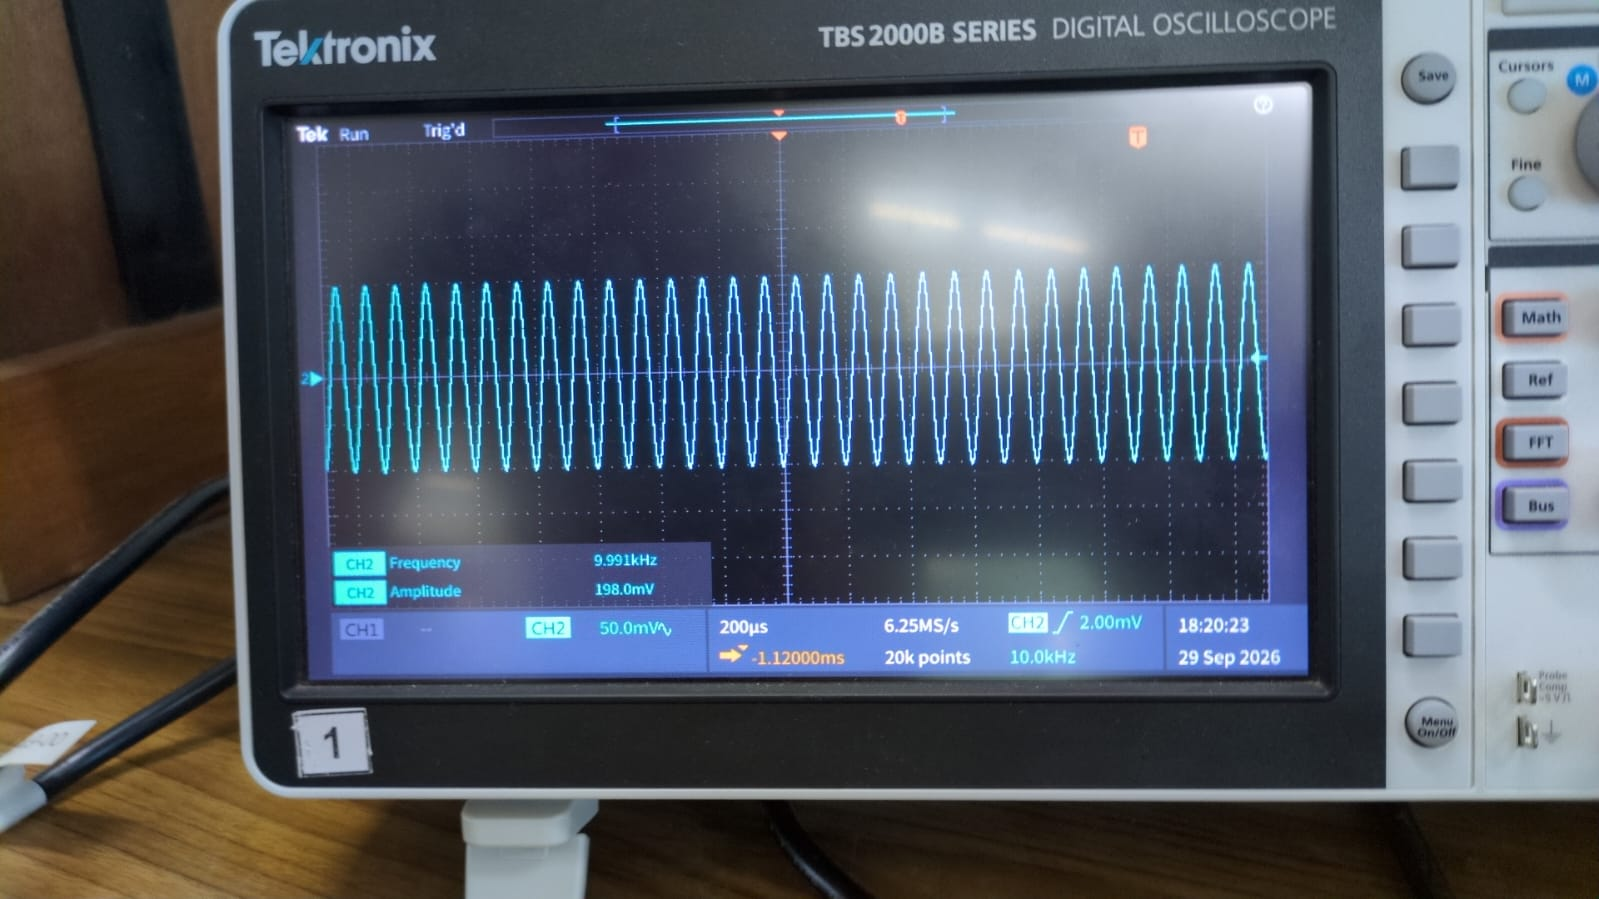
\includegraphics[height=2.5cm]{10kHz.jpeg}
        \caption{10~kHz Response.}
    \end{minipage}\\[0.4ex]
    \begin{minipage}{0.48\textwidth}
        \centering
        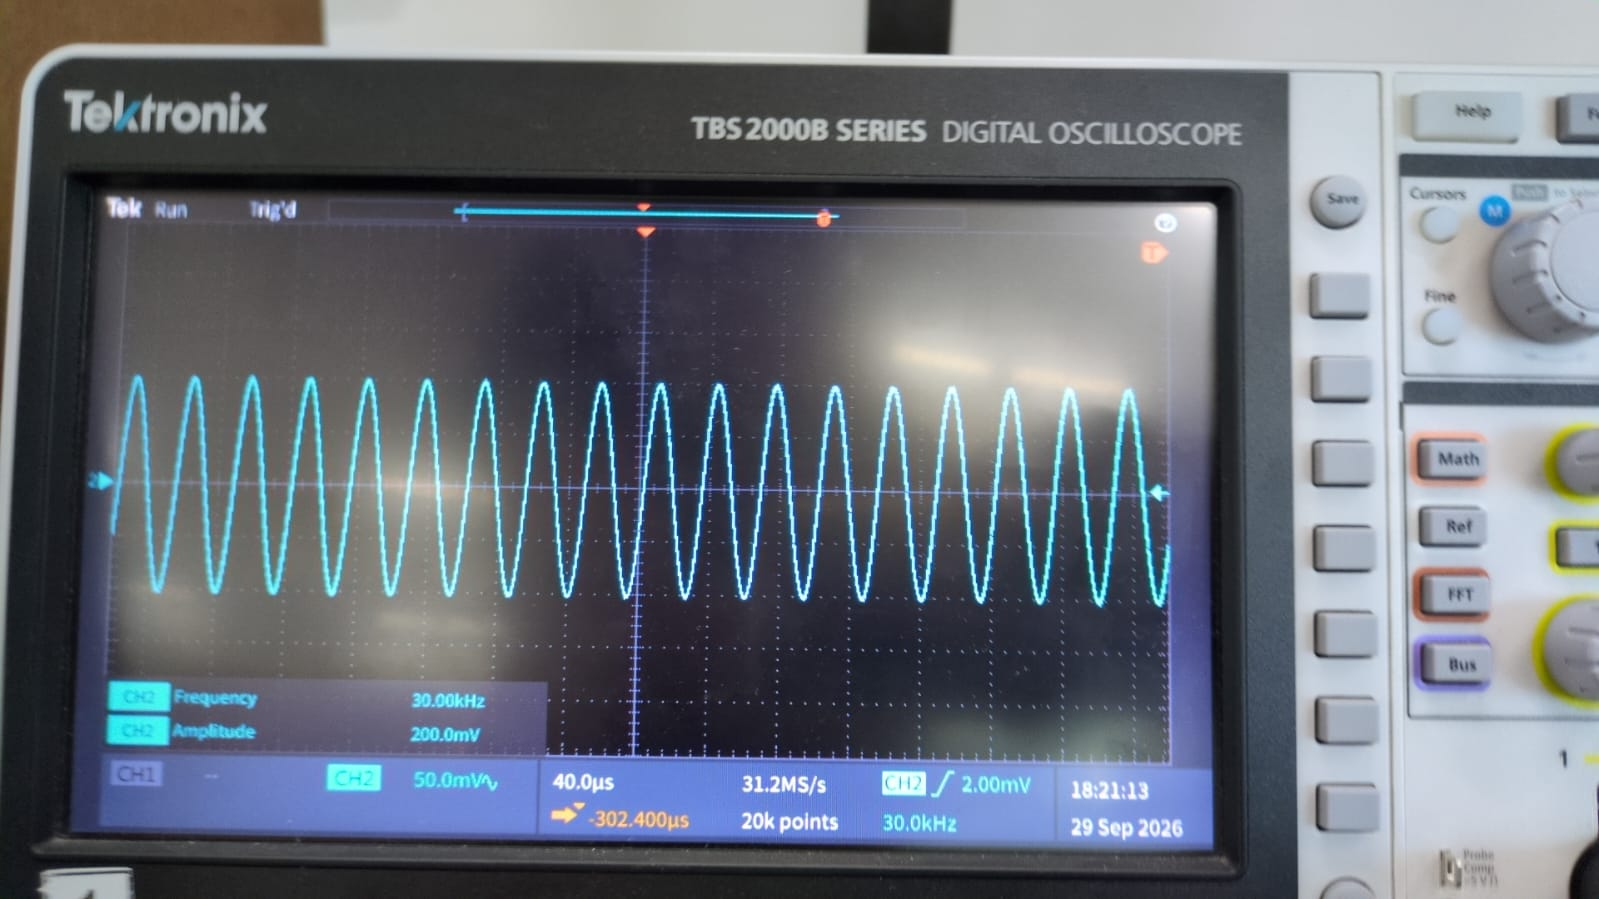
\includegraphics[height=2.5cm]{30kHz.jpeg}
        \caption{30~kHz Response.}
    \end{minipage}\hfill
    \begin{minipage}{0.48\textwidth}
        \centering
        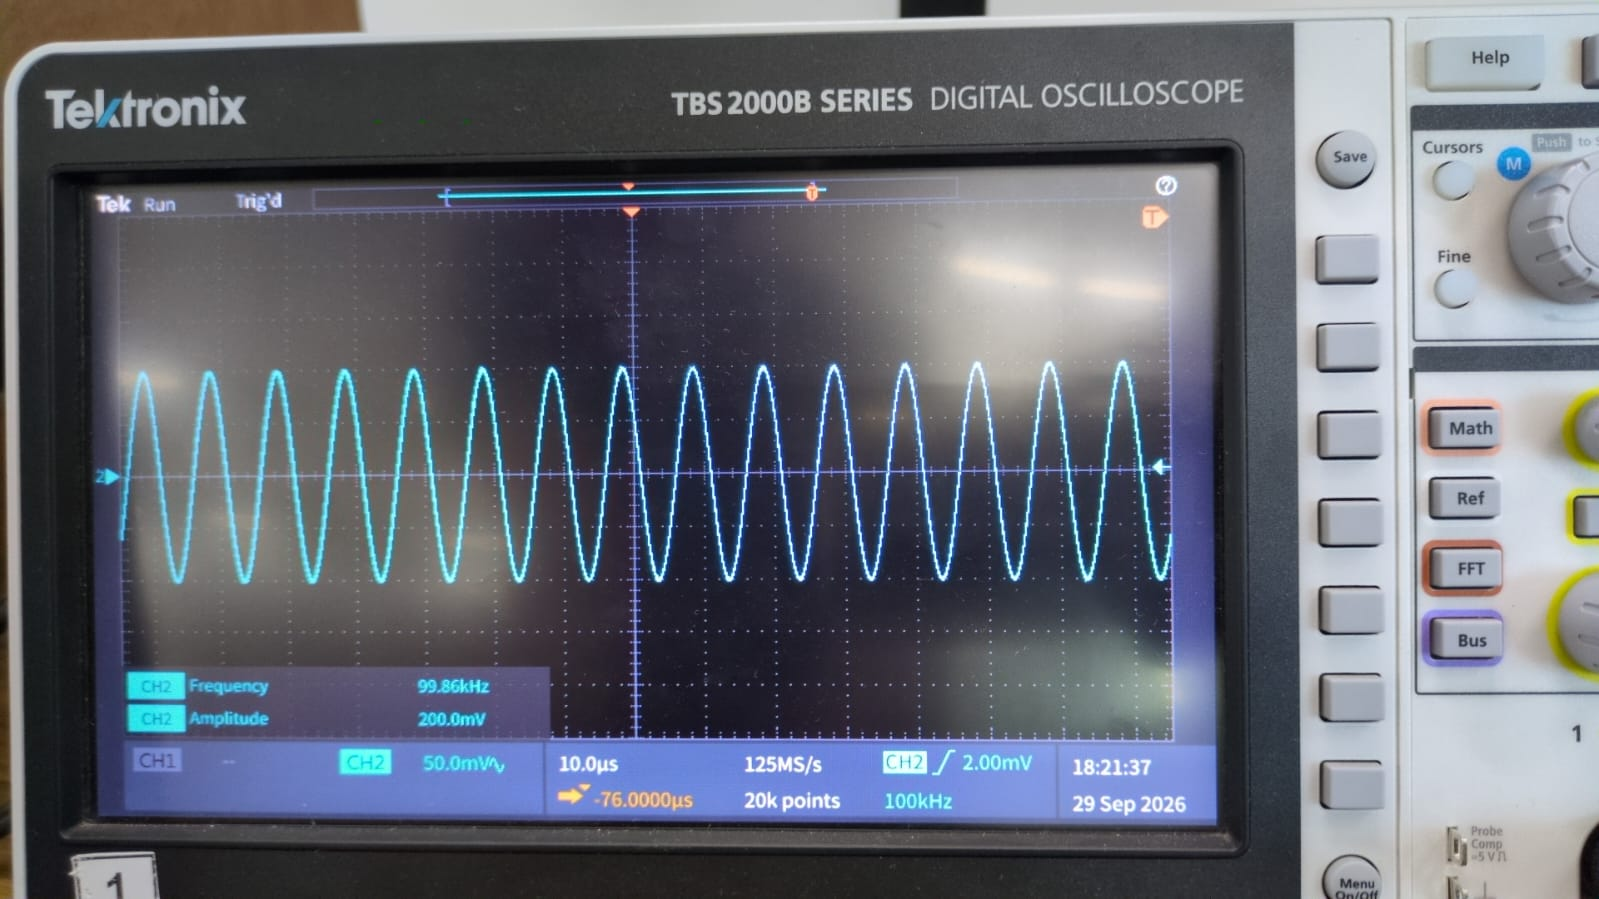
\includegraphics[height=2.5cm]{100kHz.jpeg}
        \caption{100~kHz Response.}
    \end{minipage}
\end{figure}

\clearpage
\section{Safety Precautions}
Following Section~5 and Section~11 of the laboratory manual, the following experimental and handling precautions were strictly observed:
\begin{enumerate}
    \item \textbf{ESD Protection:} Grounded handling was observed for the SI9926BDY dual-channel MOSFET breakout boards to prevent electrostatic gate-oxide puncture given the sensitive threshold ratings ($V_{GS(th)} = 0.6\text{--}1.5\text{ V}$).
    \item \textbf{Current Limiting:} The DC bench power supply current limit was engaged at $150\text{ mA}$ before connecting the circuit and remained continuously active to prevent thermal destruction.
    \item \textbf{Absolute Maximum Limits:} Maximum ratings specified on the datasheet ($V_{DS} \le 20\text{ V}$ and $V_{GS} \le \pm 12\text{ V}$) were strictly maintained under all biasing conditions.
    \item \textbf{Channel Pinout Verification:} Pin connections were verified twice against the manufacturer pinout diagram to ensure correct channel assignment ($M_{ref}$, $M_{cs}$, $M_{sf}$) across the two breakout modules.
    \item \textbf{Power Down on Reconfiguration:} The DC power supply was powered off prior to making any breadboard circuit adjustments, particularly when inserting and swapping load resistors $R_L$ during output-resistance testing.
    \item \textbf{Signal Swing Control:} Small-signal function generator amplitudes were restricted to $200\text{ mV}_{p-p}$ so that total gate voltage swings ($V_{bias} \pm V_{ac}$) remained confined within the active saturation regime.
\end{enumerate}

\section{Conclusion}
The active-loaded NMOS source follower was successfully assembled and experimentally characterized using the SI9926BDY dual MOSFET. The principal conclusions from this experiment are:
\begin{enumerate}
    \item \textbf{Wide Linear DC Tracking:} In the operating range $V_{in} = 1.5\text{ V}$ to $3.5\text{ V}$, the circuit functioned as a near-ideal voltage follower with a measured slope of $0.990\text{ V/V}$ and a level shift of $0.847\text{ V}$. Below $1.5\text{ V}$, the active mirror entered triode conduction, losing current regulation. Above $3.5\text{ V}$, simultaneous high voltage and high current produced internal Joule heating ($P \approx 0.77\text{ W}$) in the uncooled SO-8 package, initiating thermal runaway where mirror current surged above $100\text{ mA}$.
    \item \textbf{Wideband Flat Frequency Response:} Selecting $V_{in,DC} = 3.0\text{ V}$ established a thermally stable bias ($I_{cs} = 41.9\text{ mA}$) for AC testing. The voltage gain remained remarkably flat ($|A_v| = 0.980\text{ V/V}$ at 1~kHz) from 6~Hz up to 100~kHz with zero high-frequency roll-off, confirming that the follower's output pole sits well above the measurement band.
    \item \textbf{Low Output Resistance:} Capacitively coupled load tests yielded an average output resistance of $1.87\ \Omega$. This validates the theoretical promise of the weak-inversion common-drain configuration to provide very low impedance buffering ($R_{out} \approx 1/g_m$) even at modest bias currents.
\end{enumerate}

\end{document}
